%%%%%%%%%%%%%%%%%%%%%%%%%%%%%%%%%%%%%%%%%
% Masters/Doctoral Thesis 
% LaTeX Template
% Version 2.5 (27/8/17)
%
% This template was downloaded from:
% http://www.LaTeXTemplates.com
%
% Version 2.x major modifications by:
% Vel (vel@latextemplates.com)
%
% This template is based on a template by:
% Steve Gunn (http://users.ecs.soton.ac.uk/srg/softwaretools/document/templates/)
% Sunil Patel (http://www.sunilpatel.co.uk/thesis-template/)
%
% Template license:
% CC BY-NC-SA 3.0 (http://creativecommons.org/licenses/by-nc-sa/3.0/)
%
%%%%%%%%%%%%%%%%%%%%%%%%%%%%%%%%%%%%%%%%%

%----------------------------------------------------------------------------------------
%	PACKAGES AND OTHER DOCUMENT CONFIGURATIONS
%----------------------------------------------------------------------------------------

\documentclass[
12pt, % The default document font size, options: 10pt, 11pt, 12pt
oneside, % Two side (alternating margins) for binding by default, uncomment to switch to one side
english, % ngerman for German
onehalfspacing, % Single line spacing, alternatives: onehalfspacing or doublespacing
%draft, % Uncomment to enable draft mode (no pictures, no links, overfull hboxes indicated)
%nolistspacing, % If the document is onehalfspacing or doublespacing, uncomment this to set spacing in lists to single
%liststotoc, % Uncomment to add the list of figures/tables/etc to the table of contents
%toctotoc, % Uncomment to add the main table of contents to the table of contents
%parskip, % Uncomment to add space between paragraphs
%nohyperref, % Uncomment to not load the hyperref package
headsepline, % Uncomment to get a line under the header
%chapterinoneline, % Uncomment to place the chapter title next to the number on one line
%consistentlayout, % Uncomment to change the layout of the declaration, abstract and acknowledgements pages to match the default layout
]{MastersDoctoralThesis} % The class file specifying the document structure

\usepackage[utf8]{inputenc} % Required for inputting international characters
\usepackage[T1]{fontenc} % Output font encoding for international characters
\usepackage{todonotes}
\usepackage{mathpazo} % Use the Palatino font by default

\usepackage[style=numeric]{biblatex} % Use the bibtex backend with the authoryear citation style (which resembles APA)

\addbibresource{main.bib} % The filename of the bibliography

\usepackage[autostyle=true]{csquotes} % Required to generate language-dependent quotes in the bibliography

%----------------------------------------------------------------------------------------
%	MARGIN SETTINGS
%----------------------------------------------------------------------------------------

\geometry{
	paper=a4paper, % Change to letterpaper for US letter
	inner=2.5cm, % Inner margin
	outer=3.8cm, % Outer margin
	bindingoffset=.5cm, % Binding offset
	top=1.5cm, % Top margin
	bottom=1.5cm, % Bottom margin
	%showframe, % Uncomment to show how the type block is set on the page
}

%----------------------------------------------------------------------------------------
%	THESIS INFORMATION
%----------------------------------------------------------------------------------------

\thesistitle{Security through Simplicity: Implementing Secure Compartments for the MEGA65} % Your thesis title, this is used in the title and abstract, print it elsewhere with \ttitle
\supervisor{Dr. Paul \textsc{Gardner-Stephen}} % Your supervisor's name, this is used in the title page, print it elsewhere with \supname
\examiner{} % Your examiner's name, this is not currently used anywhere in the template, print it elsewhere with \examname
\degree{Bachelour of Engineering(Electronics)(Honours)} % Your degree name, this is used in the title page and abstract, print it elsewhere with \degreename
\author{Jayden \textsc{Grigg}} % Your name, this is used in the title page and abstract, print it elsewhere with \authorname
\addresses{} % Your address, this is not currently used anywhere in the template, print it elsewhere with \addressname

\subject{Electronic Engineering} % Your subject area, this is not currently used anywhere in the template, print it elsewhere with \subjectname
\keywords{} % Keywords for your thesis, this is not currently used anywhere in the template, print it elsewhere with \keywordnames
\university{\href{https://www.flinders.edu.au/}{Flinders University}} % Your university's name and URL, this is used in the title page and abstract, print it elsewhere with \univname
\department{\href{https://www.flinders.edu.au/college-science-engineering}{College of Science and Engineering}} % Your department's name and URL, this is used in the title page and abstract, print it elsewhere with \deptname
\group{\href{http://mega65.org/}{MEGA65}} % Your research group's name and URL, this is used in the title page, print it elsewhere with \groupname
\faculty{\href{}{}} % Your faculty's name and URL, this is used in the title page and abstract, print it elsewhere with \facname

\AtBeginDocument{
\hypersetup{pdftitle=\ttitle} % Set the PDF's title to your title
\hypersetup{pdfauthor=\authorname} % Set the PDF's author to your name
\hypersetup{pdfkeywords=\keywordnames} % Set the PDF's keywords to your keywords
}

\begin{document}

\frontmatter % Use roman page numbering style (i, ii, iii, iv...) for the pre-content pages

\pagestyle{plain} % Default to the plain heading style until the thesis style is called for the body content

%----------------------------------------------------------------------------------------
%	TITLE PAGE
%----------------------------------------------------------------------------------------

\begin{titlepage}
\begin{center}

\vspace*{.06\textheight}
{\scshape\LARGE \univname\par}\vspace{1.5cm} % University name
\textsc{\Large Honours Thesis}\\[0.5cm] % Thesis type

\HRule \\[0.4cm] % Horizontal line
{\huge \bfseries \ttitle\par}\vspace{0.4cm} % Thesis title
\HRule \\[1.5cm] % Horizontal line
 
\begin{minipage}[t]{0.4\textwidth}
\begin{flushleft} \large
\emph{Author:}\\
{\authorname} % Author name - remove the \href bracket to remove the link
\end{flushleft}
\end{minipage}
\begin{minipage}[t]{0.4\textwidth}
\begin{flushright} \large
\emph{Supervisor:} \\
{\supname} % Supervisor name - remove the \href bracket to remove the link  
\end{flushright}
\end{minipage}\\[3cm]
 
\vfill

\large \textit{A thesis submitted in fulfilment of the requirements\\ for the degree of \degreename}\\[0.3cm] % University requirement text
%%\groupname\\\deptname\\[2cm] % Research group name and department name
 
\vfill

{\large \today}\\[4cm] % Date
%\includegraphics{Logo} % University/department logo - uncomment to place it
 
\vfill
\end{center}
\end{titlepage}

%----------------------------------------------------------------------------------------
%	DECLARATION PAGE
%----------------------------------------------------------------------------------------

\begin{declaration}
\addchaptertocentry{\authorshipname} % Add the declaration to the table of contents
\noindent I, \authorname, declare that this thesis titled, \enquote{\ttitle} and the work presented in it are my own. I confirm that:

\begin{itemize} 
\item This work was done wholly while in candidature for a degree of \degreename.
\item This document is in accordance with the plagiarism policy of \univname.
\item Where any part of this thesis has previously been submitted for a degree or any other qualification at this University or any other institution, this has been clearly stated.
\item Where I have consulted the published work of others, this is always clearly attributed.
\item Where I have quoted from the work of others, the source is always given. With the exception of such quotations, this thesis is entirely my own work.
\item I have acknowledged all main sources of help.
\item Where the thesis is based on work done by myself jointly with others, I have made clear exactly what was done by others and what I have contributed myself.\\
\end{itemize}
 
\noindent Signed:\\
\rule[0.5em]{25em}{0.5pt} % This prints a line for the signature
 
\noindent Date:\\
\rule[0.5em]{25em}{0.5pt} % This prints a line to write the date
\end{declaration}

\cleardoublepage

%----------------------------------------------------------------------------------------
%	QUOTATION PAGE
%----------------------------------------------------------------------------------------

\vspace*{0.2\textheight}

\noindent\enquote{\itshape Strange how paranoia can link up with reality now and then.}\bigbreak

\hfill Phillip K. Dick

%----------------------------------------------------------------------------------------
%	ABSTRACT PAGE
%----------------------------------------------------------------------------------------

\begin{abstract}
  \addchaptertocentry{\abstractname} % Add the abstract to the table of contents

  Modern computers have become too complex to fully understand, let alone to fully verify.
  Therefore it has ceased to be rational to trust their security and integrity.  
  With billions of transistors and billions of lines of code, even the large corporations
  who design and manufacture computer processors and write operating systems and
  applications are unable to verify their security, as evidenced by hardware vulnerabilities
  in processors such as Spectre and MELTDOWN, and the endless stream of software security
  updates.
  In short, computers are vulnerable to attacks from the surrounding environment, and
  defence strategies are heuristic and reactionary, placing the integrity of communications
  and commerce at risk.  However this has not always been the case: The computers of the 1980s
  and early 1990s were much simpler, with software measured in kilobytes, not giga-bytes,
  and with processors with thousands, not billions of transistors.
  This thesis asks the question as to whether it is possible to create modern usable
  computing devices based on architectures so simple that they can be adequately verified
  by a determined user, and in that context, what architectural extensions might be used
  to strengthen the security of simple architectures, without making the resulting systems
  unnecessarily complex.
  A proof-of-concept system is presented based on the MEGA65 retro-computer, to which a
  robust secure compartmentalisation facility is added, together with a use-controlled
  out-of-band memory inspector, that ensures the user has complete sovereignty over the
  system, so that even were it compromised, that the compromise can be discovered and
  dealt with.

  
\end{abstract}

%----------------------------------------------------------------------------------------
%	ACKNOWLEDGEMENTS
%----------------------------------------------------------------------------------------

\begin{acknowledgements}
\addchaptertocentry{\acknowledgementname} % Add the acknowledgements to the table of contents
I would like to than Paul Gardner-Stephen for providing me with this very unique opportunity to work on the MEGA65 project as well as for his support and advice on many of the tasks that I was required to perform. I would also like to thank Tim Kirby for his previous work on the MEGA65 project, without which, the secure compartment implementation would have been impossible. In addition, I would like the thank my fellow students Lachlan McDonald and Tanguy Nodet, who helped me and worked along side me on the MEGA65.
\end{acknowledgements}

%----------------------------------------------------------------------------------------
%	LIST OF CONTENTS/FIGURES/TABLES PAGES
%----------------------------------------------------------------------------------------

\tableofcontents % Prints the main table of contents

\listoffigures % Prints the list of figures

%\listoftables % Prints the list of tables

%----------------------------------------------------------------------------------------
%	ABBREVIATIONS
%----------------------------------------------------------------------------------------

%\begin{abbreviations}{ll} % Include a list of abbreviations (a table of two columns)

%\textbf{LAH} & \textbf{L}ist \textbf{A}bbreviations \textbf{H}ere\\
%\textbf{WSF} & \textbf{W}hat (it) \textbf{S}tands \textbf{F}or\\

%\end{abbreviations}

%----------------------------------------------------------------------------------------
%	PHYSICAL CONSTANTS/OTHER DEFINITIONS
%----------------------------------------------------------------------------------------

%\begin{constants}{lr@{${}={}$}l} % The list of physical constants is a three column table

% The \SI{}{} command is provided by the siunitx package, see its documentation for instructions on how to use it

%Speed of Light & $c_{0}$ & \SI{2.99792458e8}{\meter\per\second} (exact)\\
%Constant Name & $Symbol$ & $Constant Value$ with units\\

%\end{constants}

%----------------------------------------------------------------------------------------
%	SYMBOLS
%----------------------------------------------------------------------------------------

%\begin{symbols}{lll} % Include a list of Symbols (a three column table)

%$a$ & distance & \si{\meter} \\
%$P$ & power & \si{\watt} (\si{\joule\per\second}) \\
%Symbol & Name & Unit \\

%\addlinespace % Gap to separate the Roman symbols from the Greek

%$\omega$ & angular frequency & \si{\radian} \\

%\end{symbols}

%----------------------------------------------------------------------------------------
%	DEDICATION
%----------------------------------------------------------------------------------------

%\dedicatory{For/Dedicated to/To my\ldots} 

%----------------------------------------------------------------------------------------
%	THESIS CONTENT - CHAPTERS
%----------------------------------------------------------------------------------------

\mainmatter % Begin numeric (1,2,3...) page numbering

\pagestyle{thesis} % Return the page headers back to the "thesis" style

% Include the chapters of the thesis as separate files from the Chapters folder
% Uncomment the lines as you write the chapters

% Chapter Template

\chapter{Introduction} % Main chapter title

\label{Chapter 1} % Change X to a consecutive number; for referencing this chapter elsewhere, use \ref{ChapterX}

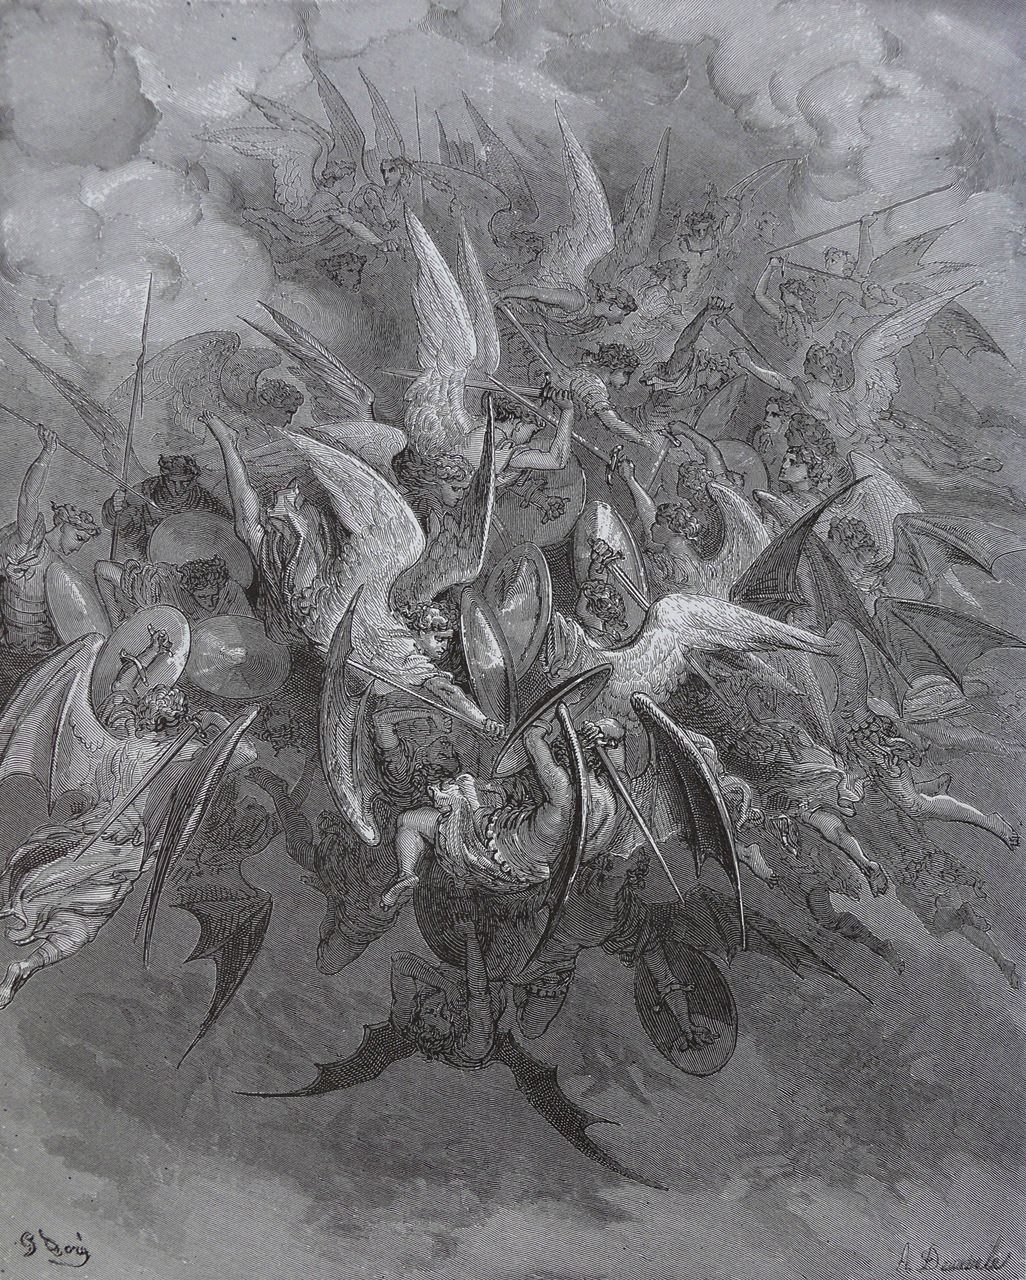
\includegraphics[width=\linewidth,trim={0 9cm 0 10cm},clip]{Paradise_Lost_24}

\section{Paradise Lost}

\label{Ch1 Sec1}

The earliest epochs of the digital era were based on a sense of control and security:  A computational device could be
created, and could be expected to behave as expected, and not to be subverted at a distance by invisible hands.
This began with the first computers that were the size of a small building, and continued until the advent of personal
computers that were capable of easy exchange of data between them, initially by floppy disk, by modem or
other forms of networking \cite{chen2004evolution}. 
Essentially, whenever a means of communications was established between computers, worms, virii and other
pathological software soon followed.   
The pathological software was initially simple in nature, and could easily be detected and removed, and into the 1990s it was not uncommon to be able to obtain anti-virus software that could detect and remove all extant pathological software from a system.
Figure \ref{fig:nortonad} shows an example advertisement from 1991, which explains that if users suspect the existence of a new virus, they can call a ''24-hour virus newsline'', betraying how relatively sedate the development and spread of computer virii was at that time.

\begin{figure}
  \centering
  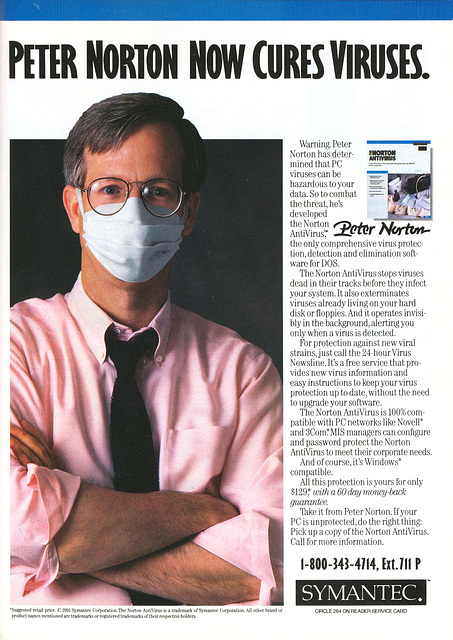
\includegraphics[width=\linewidth]{NortonAntiVirus-Advertisement}
  \caption{Early advertisement for Norton Anti-Virus for DOS. New viruses spread slowly at the time, as they could
    only be spread by floppy disk. As a result, users could be reasonably directed to call a telephone number if they
    suspected that they had a new virus on their computer. Source: \url{http://www.ipernity.com/doc/78280/6670939}.
  }
  \label{fig:nortonad}
\end{figure}

The advent of ubuiquitous internet access marked a dramatic shift:  Where as previously viruses were mostly reliant on the
movement of physical artefacts, such as floppy disks, the internet allowed for the infection of systems anywhere in the
world, without coming into physical contact \todo{Cite this}.
That is, it introduced a new and highly effective transmission mode, that was all the more insidious in that in the floppy-era
you could determine whether your computer might be at risk, based on whether it had been in contact through the insertion of
a floppy disk.
This allowed for individuals to effectively manage the sanitation of their computers in a rational and understandable manner.
The Internet allowed for invisible infection at a distance, a problem which persists to the present day, and which has created
the conditions for the wide range of malware, viruses, trojan software, ransomware, rootkits, backdoors and other pathological
software to develop and spread.

This evolution of the pathogenic material to take advantage of the available modes of delivery is directly mirrored in the
world of biology \cite{antonovics2017evolution}.
Indeed, what we see with computers now, is that the defences against these infectious threats have come to resemble the
immune system of complex animals: A variety of intrinsic protections, heuristic measures and the development of immunity only
after infection have become accepted norms for computer security.
However, this is a dangerous situation, just as animals are made sick or die or are subverted by biological pathogens, e.g., Figure \ref{fig:antzombies}), the compromise of our digital systems has significant effects for individuals and society.  And just as it is impossible to quickly
appraise whether an animal is free of all disease, it has become impossible to determine authoritatively whether a computer
is free of all digital pathogens.

\begin{figure}
  \centering
  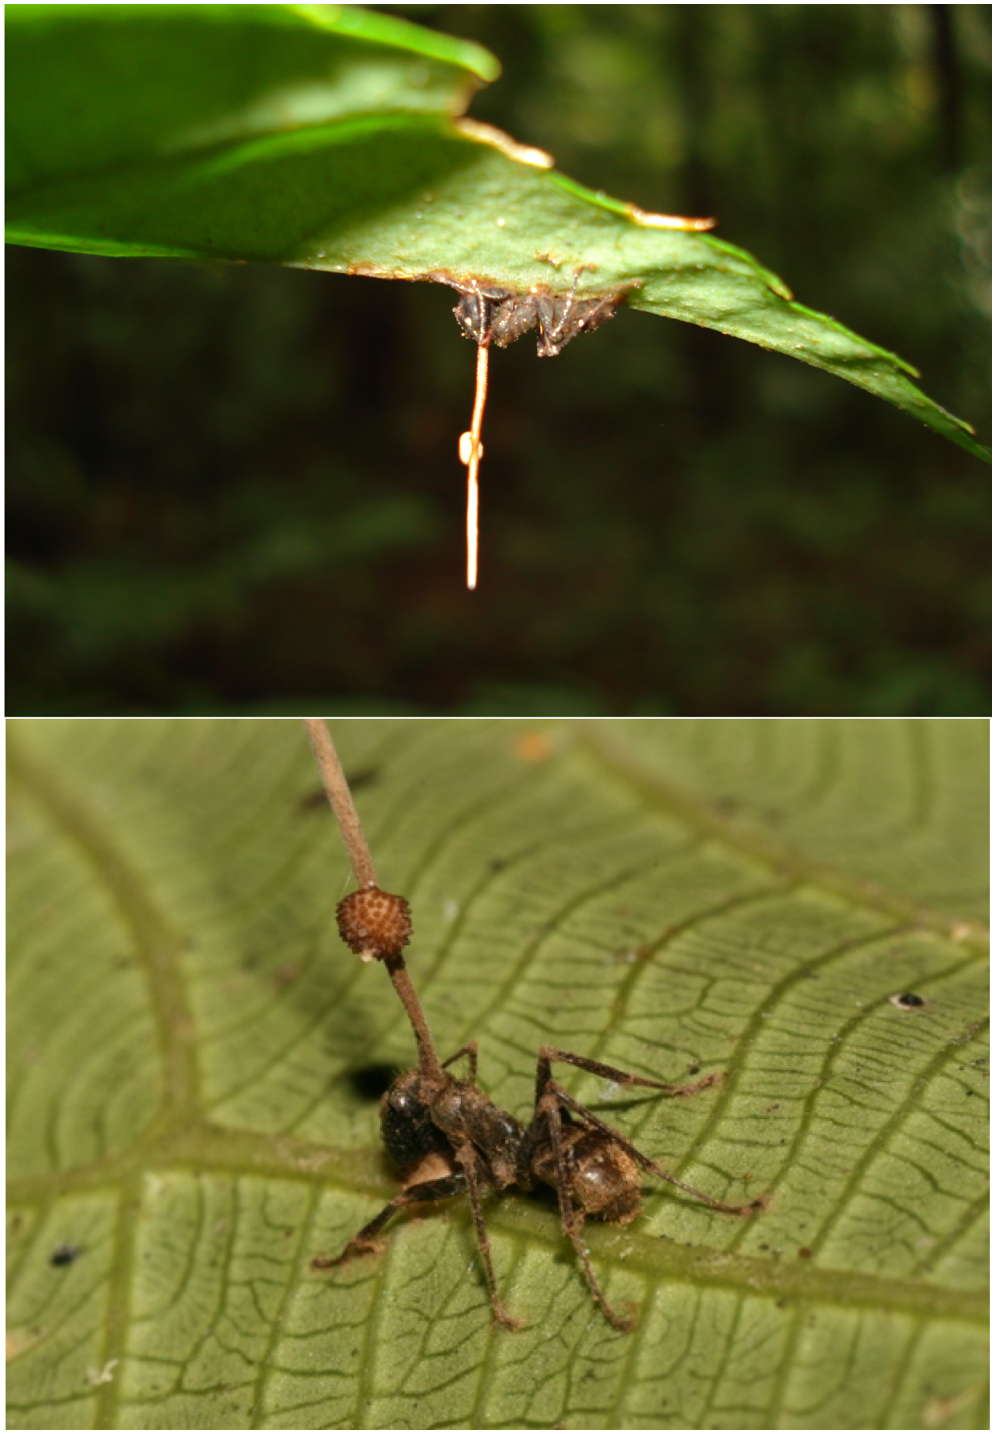
\includegraphics[width=0.8\linewidth]{Ophiocordyceps_unilateralis}
  \caption{
    {\em Ophiocordyceps unilateralis} is perhaps better known as the ``zombie ant fungus''.  When it infects an ant,
    it modifies the ant's behaviour, so that it leaves its ground-based nest-mates, climbs a tree and finds a leaf,
    and bites into the underside of the leaf so that it hangs upside down. Several days later the fungus emerges from
    the head of the ant in a fruiting body that showers its nest-mates with spores, thus spreading quickly through
    entire colonies.  Source: 
    \url{https://upload.wikimedia.org/wikipedia/commons/8/85/Ophiocordyceps_unilateralis.png}
    \label{fig:antzombies}
  }
    
\end{figure}

Not only are there connections between pathogens and computer viruses in general, but eeriely enough, there are some computer viruses that behave almost identically to a biological counterpart. 
The Intel management engine is a small CPU that has been in almost all Intel chips for the past 18 years. 
Late in 2017, a proof of concept subversion on the Intel management engine was done by Mark Ermolov and Maxim Goryachy \cite{Hackaday}. In this subversion, the engine was proved to be directly controlable with out being visible to the user, meaning that a hacker could potentially cause your machine to attack itself. 
This is the equivalent of an auto-immiune disease in the biological world, as the greater organism, whether that is man or machine, is being attacked by part of itself. 
The parallels do not stop here however, HIV/AIDS are immune system weakening diseases. 
These diseases are often not the cause of death themselves, but are often contributers \cite{ggHIV}. 
Much like these diseases, the "BadBIOS" phenomenon does not directly cause the death of a computer. 
This virus instead secretly and with out user authorisation, opens the communication channels of any computer it infects \cite{Reference5}. 
The similarities between "BadBIOS" and HIV/AIDS does not stop there, both are extremely resistant to treatment to the point where they are almost permanant. 
In the case of "BadBIOS" this infects the main program that controls all the actions of the computer. 
Because all other operations occur on the computer through this master program, there is no way to remove all of the infection which could be lurking anywhere \cite{Reference5}.

Were this not depressing enough, the problem is complicated by the fact that computers have, like biological organisms,
become so complex, that it is impossible to construct them in such a way that they can effectively resist being subverted.
The interactions in modern software are now so rich -- like the interactions of proteins, genes and other elements that make up
the control machinery of living cells -- that it is impossible to fully understand them in all but the most trivial of circumstances.

This problem has been compounded by Moore's Law \cite{Moore}, which has made it cheaper to create ever more complex computers, and
by human psychology which have created an emphasis on the number of features or functions of a given piece of software, rather than
on its correctness and security.  
Thus software has exploded in size from kilo-bytes in the early 1980s to tens of giga-bytes in the current era. 
That is, software is now often millions of times larger and more complex than it once was, to the point where verification of correctness has become effectively impossible.

As bad as this situation is for software, it is even worse when hardware systems are considered, and the central processing units
(CPUs) of computers in particular.  
CPUs have also grown in complexity from thousands of transistors to tens of billions of transistors over the same time period.  
However, unlike a defect in software, a defect in a CPU cannot necessarily be corrected without physical replacement.

The fact that the Spectre and MELTDOWN vulnerabilities existed in CPUs for almost 20 years before being discovered \cite{Spectacular}
is strong evidence that we have long since passed the point where even a well-resourced company like Intel or AMD can ensure
the correct operation of a CPU.  
If these companies with many thousands of verification engineers cannot achieve it, what hope do individuals and small organisations have for verifying the correct operation of their computing devices?

What is clear is that the problem is one of complexity: A single transistor can be easily verified. The simple early CPU designs
like the 6502, that consisted of only a few thousand transistors can also be easily verified.  But modern complex CPU designs cannot.
There must exist somewhere a tipping point where verification ceases to be realistic for a determined user.
Beyond that point security is merely a hopeful dream, because we can no longer prove correctness and immunity to the challenges
that it might face, just as avoiding the common cold is also no more than a hopeful dream, and certainly nothing that can
be guaranteed if we are to remain in communications with the outside world.

We are therefore forced to accept the unpalatable truth that we are no more sovereign over our computing devices than our bodies
are over the biological world that surrounds us: We have been cast from the Eden of security for eating the forbidden fruit of
ever increasing complexity and functionality.

The question is whether we can go back, to create computing devices that are sufficiently simple as to be securable, and yet
remain sufficiently useful in practice.  This is the motivating question for this thesis.

\section{Research Questions}

\label{Ch1 Sec2}

\textit{What are the missing or non-functional sub-systems that the MEGA65 requires to be implemented?}\\
Which will be answered in the form of a survey of the current sub-systems of the MEGA65, and a survey of the sub-systems required to create a functional prototype.\\
\\
\textit{How can these sub-systems be implemented?}\\
Which will be answered by the creation of plans for the implementing of the missing or incomplete sub-systems.\\
\\
\textit{How can the simplicity, understandability and hence, the security of these sub-systems be maximised?}\\
Which will be answered by considering each sub-system, qualitatively appraising its simplicity, understandability and security, and where appropriate, making well researched recommendations for refining those components to improve one or more of these axes, and time permitting, acting on those recommendations.\\
\\
\textit{How can the complete MEGA65 architecture be physically prototyped on the bench?}\\
Which will be answered by examination of the current partial bench prototype and comparing it with the sub-systems identified through the other research questions, and designing and realising a complete bench prototype.
This will occur through coordination with Mr. Lachlan McDonald, who is undertaking the designing of the PCB for the MEGA65 smart-phone device.\\
\\
\textit{How can the secure compartmentalisation's architecture planned for the MEGA65 be realised?}\\
Which will be answered by considering this architecture and the current state of the MEGA65 system to derive and execute a method for implementing a secure compartmentalisation architecture.\\
\\
Overall the success of the project will be measured against the creation of a functioning bench prototype device that, through the architecture, implements the secure and understandable compartmentalisation of hardware to the point of demonstrability.

%----------------------------------------------------------------------------------------
%	SECTION 3
%----------------------------------------------------------------------------------------

\section{Thesis Layout}

\label{Ch1 Sec3}

Following this chapter, "Chapter \ref{Chapter 1} : Introduction", is the chapter, "Chapter \ref{Chapter 2} : Literature Review".
In which relevant background information regarding complexity and cyber security, mobile devices, isolative security and the MEGA65 project will be given.
After this, "Chapter \ref{Chapter 3} : Methods and Materials" will go on to describe how this project was undertaken and what tools were used.
This will be immediately followed by "Chapter \ref{Chapter 4} : Project Set-up".
In this chapter, details about the issues faced immediately after joining the project will be made clear.
Following this is "Chapter \ref{Chapter 5} : Matrix Mode Corrections", in this chapter the issues encountered with the matrix mode and their fixes will be made clear.
"Chapter \ref{Chapter 6} : Secure Compartmentalisation" will follow, in which an overview of how the secure containers in the phone were implemented will be given.
This will be followed by "Chapter \ref{Chapter 7} : Results and Discussion" where the challenges, what was achieved and research questions will be talked about. In addition to this, the future works for the secure compartment and matrix mode portions of the project will be outlined.
Finally, "Chapter \ref{Chapter 8} : Conclusion" will discuss the various details about the findings of this document, as well as answers to the research questions outlined in section \ref{Ch1 Sec2}.


% Chapter Template

\chapter{Literature Review} % Main chapter title

\label{Chapter 2} % Change X to a consecutive number; for referencing this chapter elsewhere, use \ref{ChapterX}

Since the introduction of general-purpose mobile operating systems, such as Symbian, Android, Windows 10 and iOS, and especially throughout the last decade, mobile phones have evolved dramatically.\cite{Reference1}
The introduction of feature-rich and complex operating system has not only brought the benefits of a computer, but also the risks of one too.\cite{Reference2}
Since phones have become computerised people have become more trusting of what data they can store on their phone, such as location, bank details, etc.\cite{Reference3}
With private data increasingly being stored on phones, it becomes necessary for mobile security to receive a larger amount of attention.
This literature review explores this issue, as follows: Section \ref{Ch2 Sec1} explores the interrelationship between complexity and security, Section \ref{Ch2 Sec2} documents a wide variety of the security threats facing modern computers, with a particular emphasis on mobile devices, Section \ref{Ch2 Sec3} relates the application of isolation and compartmentalisation to improve security, and Section \ref{Ch2 Sec4} documents the history and status of the MEGA65 project, including the historical Commodore 64 platform on which it is based, as well as the recent work towards introducing compartmentalisation and related 
security features to the platform.\todo{This is a monster sentence\!}

%----------------------------------------------------------------------------------------
%	SECTION 1
%----------------------------------------------------------------------------------------

\section{Complexity and Security}

\label{Ch2 Sec1}

One of the major issues with the current state of security is that the complexity involved is far beyond what any one person can comprehend.
Intel embodies the complexity issue perfectly when examining the number of employees vs the number of transistors on one of their CPUs.\\

\begin{figure}
  \centering
  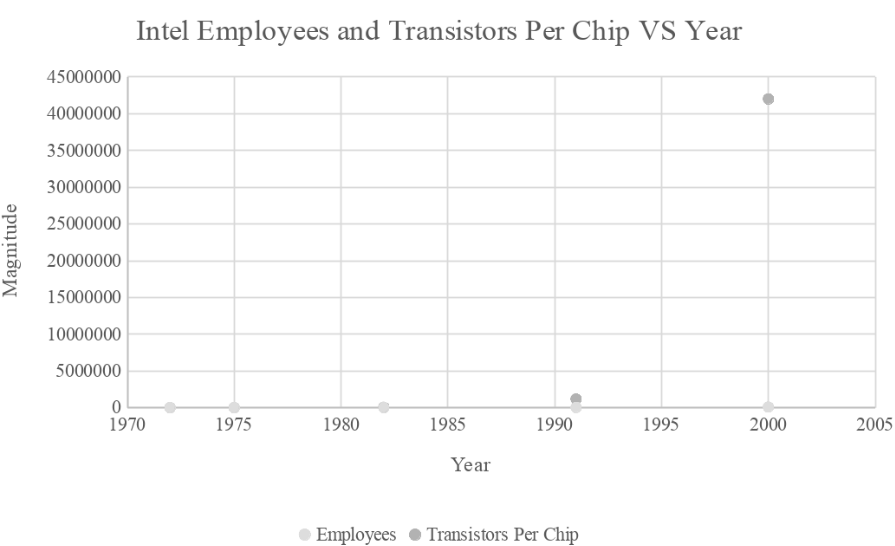
\includegraphics[width=\linewidth]{intelgraph}
  \caption{Graph of Intel's CPU transistor count vs the amount of Intel employees.\\ \cite{Reference28}\cite{Reference29}\cite{Reference30}\cite{Reference31}\cite{Reference32}\cite{Reference33}\cite{Reference34}\cite{Reference35}
}
  \label{fig:intelgraph}
\end{figure}

From 1972 to 2000 Intel’s workforce grew by 86 times, comparing this growth with the transistor growth of 1200 times over the same period, a huge disparity can be seen.
If every employee at Intel was dedicated to testing transistors, in 1972 each employee needed to test 3.5 transistors, compare this to the 487 they need to test now.
This clearly demonstrates the impossibility for, not only one person, but for all of Intel to successfully verify that their CPU is working as intended.
With modern computers unable to be understood by a single person, they are inherently not to be trusted.\cite{Reference4}\todo{references should go before the full stop. You need to change this in lots of places.}
Not only are they not to be trusted, but they can never be trusted, because while they are not understood by a single person there is always the possibility of interactions in the CPU that remain undiscovered.\cite{Reference5}\\
As systems become more complex, they too see more issues arise within them.
A key property of this is the amount of failure modes that are present in the system.
Larger, more complex, systems naturally have more security vulnerabilities as they have more interactions, or opportunities for failure.\cite{Reference6}
These larger systems also require more time and effort to test.
More worryingly is that for the end user, this complexity aids malicious attempts.\cite{Reference7}
For the same reasons that testing is difficult, so too is finding indicators of a security breach, or even malicious activity after a breach has been detected.\cite{Reference8}\\
To combat this increase in security flaws there are a few methods that can be used.
One such method is to patch the security flaws with work-arounds.
As these work-arounds were not originally designed as part of the system, there is a possibility that they can make the entire system less secure overall.\\ 
This has been beautifully demonstrated by the recent exploits found in speculative execution processors.
This exploit, named Meltdown, was a massive cause of panic as it allowed privileged information to be read at megabytes a second.
The Windows 7 January 2018 patch for the exploit resulted in permissions for the user being set erroneously.
This allowed the user to read memory that was normally only accessible by the processor.\cite{Reference9}\\
The other method of reducing security flaws is to reduce the complexity of the system.
Less interactions allows more time dedicated to ensuring each one works correctly.
In addition to this, simpler systems allow for users to better understand them, and thus are more easily verified as secure.
This was listed as one of the key aspects of a trusted computer system by the Department of Defence as it is only then that understandable and maintainable protection is achieved.\cite{Reference10}

%----------------------------------------------------------------------------------------
%	SECTION 2
%----------------------------------------------------------------------------------------

\section{Mobile Security Threats}

\label{Ch2 Sec2}

When analysing current mobile (smart) phones there are multiple avenues under which data can be maliciously obtained, or normal service can be disrupted.
These avenues can be categorised under the following labels:
\begin{itemize} 
\item Mobile Hardware
\item Mobile Software
\item Mobile Networks
\item Physical Access
\item Mobile Enterprise 
\end{itemize}

%-----------------------------------
%	SUBSECTION 1
%-----------------------------------

\subsection{Mobile Hardware}

\label{Ch2 Sec2 Sub1}

Mobile hardware refers to the various sensors and physical devices built into the phone.
By accessing the hardware directly on the phone, most software security provided by the operating system is bypassed, allowing malicious users to access data provided by cameras, microphones, etc.
This form of attack is particularly difficult to protect against in some cases due to the advent of users rooting or jail-breaking their phones.\cite{Reference11}
Jail-breaking/rooting is where the user deliberately uses exploits vulnerabilities to gain more control over the phone’s systems.\\
Currently, the best way to defend against mobile hardware exploitation is to ensure that the operating system is up to date and that patches for publicly known exploits are installed.
This does not prevent mobile hardware exploits but rather makes them nontrivial to perform.\cite{Reference12}\\
Even with all the updates and patches installed, there still exists improvements that could be made to further reduce hardware exploits.
As most hardware on a phone does not have an indicator for when it is active, it is difficult to determine its status; implementing this in hardware would allow a user to tell decisively whether hardware was on or off.\cite{Reference13}

%-----------------------------------
%	SUBSECTION 2
%-----------------------------------

\subsection{Mobile Software}

\label{Ch2 Sec2 Sub2}

Mobile software refers mainly to the applications running on the phone, but it  also refers to the background processes that run while the user isn't using their phone.
While these programs give the user more control over their phone, they are also a potential source for coding errors.\\ 
Through these errors such as, files being stored in an unprotected location or files being stored in an insecure format, it is possible to leak sensitive data.\cite{Reference14}
Not only is it possible to read stored data, but through an insecure network or a vulnerable third-party software library, it is possible to read and alter all data being sent to and from the phone.\\ 
To protect against vulnerable software there are limited options available.
Keeping the operating system up to date is the best solution as more security monitoring helps catch exploits.\cite{Reference12}
The process of application analysis involves two different methods, static analysis and dynamic analysis.
In static analysis the source code for an application is evaluated without running it to detect possible exploits.
This method relies on the source code being available, which isn’t always the case, and, if it is computer assisted, can provide false positives.\cite{Reference15}
To a lesser extent, static analysis can be performed on compiled code, but it is limited to program interface, compiler optimisations and software library checking.
Dynamic analysis is like source code static analysis with the exception that it is done with the code running.
This allows behaviour that is not apparent from source code examination to be identified.\cite{Reference13}\\
In addition to coding errors that allow third parties to exploit security vulnerabilities, some applications are developed intentionally for malicious activity.
These less than reputable applications often exploit underlying vulnerabilities in the operating system or trick the user into giving the application privileges that exceed those needed for proper function.\cite{Reference16}\\
Malicious applications can breach phone security in many ways to extort money from the user or gain access to protected data.
Ransomware is the name given to an application that encrypts all the user’s data and demands payment to decrypt it.
This form of extortion poses extreme risk when dealing with cooperate data due to the loss in productivity.
The unauthorised access of user data can be done through many methods such as jail-breaking the phone so that hardware can be exploited, subverting login details, sharing data with other applications (such as Dropbox) and logging private data.\cite{Reference13}\\
Malicious applications are difficult to protect against.
In almost all situations they require some form of active security that is user reliant to effectively protect against them.
In addition to understanding the threats present and keeping all software up to date, users can:\\*
\begin{itemize}
\item Use dynamic analysis in a safe environment
\item Isolate the application from sensitive data
\item Use authentication protocols
\end{itemize}
These methods would allow for adequate protection against malicious applications or applications used for a malicious purpose, but there is still more that can be done.
Better application development practices and regulations would prevent many of the issues with software exploitation.
This is unrealistic though as most applications are so complex there will always be a missed bug.
More transparent applications are the solution to this as it would allow users to not only verify the application but improve upon it.\cite{Reference13}

%-----------------------------------
%	SUBSECTION 3
%-----------------------------------

\subsection{Mobile Networks}

\label{Ch2 Sec2 Sub3}

A mobile network is the interconnection between all phones that allows for phone calls, messages and internet access to the mobile device.
These connections are facilitated by the numerous radios and modem.
The mobile network can be broken down into three major sections, the radio access network, the core network and the external services network.\\
The radio access network facilitates the connection between the mobile device and the service provider for the phone.
This network is used to connect the mobile device to the telephone tower which then leads to the core network.
The core network is responsible for tracking billing, signal routing and connecting the mobile device to the external services network, such as the internet or mobile devices from a different carrier.\cite{Reference13}\\ 
Radio access networks are susceptible to three basic types of exploits, denial of service attacks, eavesdropping and device tracking.
Denial of service attacks is used as a large umbrella term for all the attacks that can block or hinder normal mobile phone operation.
These attacks can be conducted by filling up all available radio access slots on a telephone tower, impersonating a telephone tower to intercept emergency calls or flooding the area with radio waves to obscure legitimate calls.\cite{Reference17}
Eavesdropping, as the name suggests, involves the gaining access to data being transmitted between the telephone tower and mobile device.
This is possible because it is not required that data between the mobile device and the telephone tower be encrypted, in the case that end to end encryption is not used, all the user’s data is free to access by those that can.\cite{Reference13}
For superior data transmission a shorter radio access network is desired, this bring forth a need for mobile device locational services, so the closest radio tower can be used in data transfer.
This can be exploited to track a mobile device and by extension, a user’s location.\cite{Reference17}\\
The core network, once subverted, offers attackers many avenues of attack.
Most mobile networks use some form of management system in order to control the entire network.
This provides the ability to intercept or block phone calls and texts, as well as denying service to users were it subverted.\cite{Reference13}\\
External networks are how a phone connects to the internet among other networks.
This brings all the benefits, but also all the dangers of an internet connection.\\
To defend against data interception and theft, end to end encryption must be used.
This negates any chance of the radio access network and core network leaking data, as the leaked data would still be encrypted.
Denial of service attacks can be mitigated by alternative methods of data transmission.
Though it is highly unlikely that an entire carrier will have it’s services denied, using an alternative method would be able to negate any and all effects of such an attack.
Unfortunately, mobile device tracking cannot be defended against due to it being so intertwined with the mobile network.
Even bouncing a connection across a privately-owned network would not result in much, as it can be traced by a skilled attacker.\cite{Reference13}

%-----------------------------------
%	SUBSECTION 4
%-----------------------------------

\subsection{Physical Access}

\label{Ch2 Sec2 Sub4}

While mobile phones are almost always on person all the time, there are certain situations in which contact must be broken.
These instances occur during certain security checks, like police or airport searches, or during charging and communication sensitive operations.
During these times it would be possible to access data from the phone or perform other malicious activity.\\
One avenue of attack is the combined charging/data port of the phone.
By plugging the phone into a PC, it is possible to abuse vulnerabilities to gain access to data.
This is not limited to PCs however, by modifying a charger with a small PC board it is possible to execute complex attacks on the device whenever the phone is charging.
If done right, this attack could also work in the reverse, infecting a host computer that the phone is connected to.\cite{Reference13}\\
Another avenue is the phone itself, NowSecure released a report in 2016 that stated 43\% of mobile users do not use a pass-code, PIN, or pattern lock on their device.\cite{Reference18}
This, coupled with cached memory and browser cookies could result in banking details, among other things being stolen.\\

The best defence against physical access attacks is to use screen locks and exclusively use personal charging equipment.
These negate the threat of physical access attacks and data port attacks.\\

Despite the ease of ensuring physical security, more needs to be done to encourage users to use this security.
Currently, most phones use authentication methods that don’t fully capitalise on all the mobile sensors available.
While using sensors like fingerprint scanners and facial recognition is emerging in mobile phones, there exists sensors like the capacitive sensor, gyroscope and accelerometer that are still unused in lock screen technology.[\cite{Reference13}

%-----------------------------------
%	SUBSECTION 5
%-----------------------------------

\subsection{Mobile Enterprise}

\label{Ch2 Sec2 Sub5}

When mobile devices are integrated into business there comes a need for servers, processes and systems that manage these devices.
This enterprise, such as a company application, can serve as an infection source, should the enterprise itself become infected.
To counteract these flaws mobile device managers for enterprise purposes have been developed.
These managers enforce security policies, remote access, remote wiping, etc. for the device.\\
Because these device managers have a higher level of privilege than the user, exploiting the device manager to gain access to the entire enterprise is a serious threat, as doing so would allow infection of all devices connected to the enterprise.
Once compromised, it is possible for all data within the enterprise to be stolen, manipulated or for all services to be blocked completely.\\
These attacks can be mitigated using comprehensive authentication protocols to prevent impersonation, protected execution environments and network monitoring.
While authentication prevents most forms of attack, it is still subject to authentication information being discovered, which is why the execution environment is used to contain malicious activity and network monitoring is used to look for such activity.\cite{Reference13}

%----------------------------------------------------------------------------------------
%	SECTION 3
%----------------------------------------------------------------------------------------

\section{Security Through Isolation}

\label{Ch2 Sec3}

One approach to securing a computer has been to have sections of it “air gapped”, such that infection in one area cannot affect other areas.\cite{Reference19}\\

One example of an operating system built on this principle is the Qubes OS, which has gone about this through compartmentalisation.
By isolating things, such as untrusted websites, in their own qube it is possible stop any attempt to compromise the whole system as they are contained in that qube.
These qubes are not limited to software, they work with hardware too, meaning that USB controllers and network cards are secured in their own qubes.
This reduces the effectiveness of using hardware as a security exploit.\cite{Reference20}\\

Isolative computing can be emulated by hosting multiple virtual machines on one host machine, thus recreating the Qubes OS concept.
This comes one major disadvantage over using Qubes OS however, once the host OS is subverted all the virtual machines are subverted too.\cite{Reference21}
As Qubes OS uses a hyper-visor to manage all the qubes it is inherently more secure than virtual machine recreation.
This is due to the increased difficulty of subverting the hyper-visor as compared to subverting an operating system.\\

Another method for air gapping a computer is to have it physically isolated from external connections.
By removing the computer from external networks almost all attack vectors are removed too, thus ensuring the computer is safe.
This form of protection is mainly used in critical systems, as by isolating a computer a lot of the functionality of it, such as web browsing, is removed.\cite{Reference22}\\

While air gapping computers appears to make data exfiltration impossible, there are a few ways in which this can happen.
The simplest method is via physical access and a USB or USB device.
The best know device is the USB Rubber Ducky, this device can be used to imitate a keyboard inputs via a script loaded onto the device.\cite{Reference23}
This allows the rubber ducky full control over the host device and can even be used to install malicious software.\cite{Reference23}
Another method of circumventing an air gap is to use high frequency sound from a speaker to transmit and infect air gapped computers\cite{Reference24} “AirHopper” is another method for data exfiltration, instead of using sound, it uses radio waves generated by cables from the computer.\cite{Reference25}
Even when Faraday shielded to prevent these sound and electromagnetic signals from escaping, it is still possible to transmit data from the computer by using the CPU.
The CPU can be used to generate low frequency magnetic waves by altering the load on specific cores.
These magnetic waves more readily penetrate Faraday shielding, allowing the transmission of data from the air gapped computer.\cite{Reference26}

%----------------------------------------------------------------------------------------
%	SECTION 4
%----------------------------------------------------------------------------------------

\section{The MEGA65 Project}

\label{Ch2 Sec4}

The MEGA65 project was born from one Paul Gardner-Stephen in 2014.
The scope of the project was to create an accelerator for the commodore 64.
This changed when the Museum of Electronic Games and Art sponsored the project and connected him with various other experts.\cite{Reference27}
The project was expanded to recreating and archiving the commodore 65, a prototype computer that was never officially released.
In addition to the restoration of this computer, updating the hardware was done wherever possible, so long as they didn’t compromise the identity of the computer.\cite{Reference27}
This was done so an external accelerator was not needed for the project.\\

The MEGA65 computer itself runs on a field programmable gate array (FPGA) dev board.
This option was explored in depth due to a few factors such as, cost, onboard SD card slot, VGA output and the Artix-7 chip.
The cost of boards was a large factor in the decision to use them as they would make the C65 affordable.
The SD card slot on the board also helped this affordability as they are inexpensive and, conveniently, able to easily be interfaced with many computers.
The VGA interface on the board was considered noteworthy as many monitors still have a port for them and there are readily available adaptors for VGA to various other ports.\cite{Reference27}\\

In addition to the MEGA65 project, another project was run along side it, the MEGAphone project.
This project aimed to create a commodore 65 based smart phone with a security focus.
Instead of allowing the technology gap between the MEGAphone and modern phones to be detrimental, it would be one of the key features of the phone.
The vastly simplified way in which the computer worked as well as the age would allow for many advantages over modern systems.\\

The simplicity would allow for the entire device to be verifiable, this is not normally explored by other security development teams.
By being able to verify the phone is working as intended, it becomes almost impossible to compromise.
In addition to this, as the phone is security focused, malicious activity is limited by the phone design itself.
Not only this, but many of the security flaws being found in systems today are just not present in the commodore 64 because it doesn’t have the supporting hardware.

Through the 36 years of activity that the commodore 64 has seen, many bugs have been found and documented in the system.
As such, it is monumentally unlikely that there are new exploits in the system that are unfound, making it excellent to use for security purposes.

 
% Chapter Template

\chapter{Methods and Materials} % Main chapter title

\label{Chapter 3} % Change X to a consecutive number; for referencing this chapter elsewhere, use \ref{ChapterX}

This chapter describes how work on the project was conducted. It does this by first describing the methodology used, then by following with the hardware and software used.

%----------------------------------------------------------------------------------------
%	SECTION 1
%----------------------------------------------------------------------------------------

\section{Methodology}

\label{Ch3 Sec1}

This project included several states, in which, debugging skills and a deep programming knowledge base was necessary. While debugging there were a few techniques used that enabled fast and more accurate pinpointing of the offending pieces of hardware. Chief among these debugging techniques was to visually expose relevant signals. By exposing a signal in real time it could be quickly and easily verified as either working or not working. Should this fail, another useful debugging technique was to simulate the modules with report statements. While this was not always viable, it did allow for much more real time data to be exposed; it also allowed exact inputs to the hardware to be monitored. The final debugging technique used was to reduce the complexity of the hardware. By removing more complex elements of the hardware it is possible to isolate the issue and then fix it.

\section{Materials}

\label{Ch3 Sec2}

%-----------------------------------
%	SUBSECTION 1
%-----------------------------------
\subsection{Hardware Used}

\label{Ch3 Sec2 Sub1}

During the development of the project several pieces of hardware was used, this hardware was used to create interact and program the MEGA65. In addition to this some of the work on the project required specific hardware to function in order for full functionality of the MEGA65 to be present. This hardware is listed as follows:\\

\begin{itemize}
\item{Digilent Nexys 4 DDR Artix-7 FPGA Trainer Board: This FPGA development board, as seen in figure \ref{fig:nexys4ddr}, was one of the vital components while conducting this project. It was used as the remappable hardware, on which, the MEGA65 prototypes could be tested.}
\item{Acer Aspire V Nitro: This laptop, as seen in figure \ref{fig:aspirevnitro}, was the most important piece of hardware used in this project. This piece of hardware was used to interface between the FPGA as well as make changes to the MEGA65 hardware.}
\item{Dell UltraSharp 2408WFP 24-inch LCD Monitor: This monitor, while not critical, was a required piece of hardware. This was used to host the VGA output from the MEGA65.}
\item{Dell KB1421 Keyboard: Much like the monitor, this piece of hardware was not critical but without it, or a similar product, progress on the project would be exceedingly difficult.}
\item{SanDisk Ultra 16Gb MicroSDHC Micro SD card: This SD card, like the keyboard and monitor, was not critical, it was necessary for full operation of the MEGA65 however.}
\end{itemize}

\begin{figure}
  \centering
  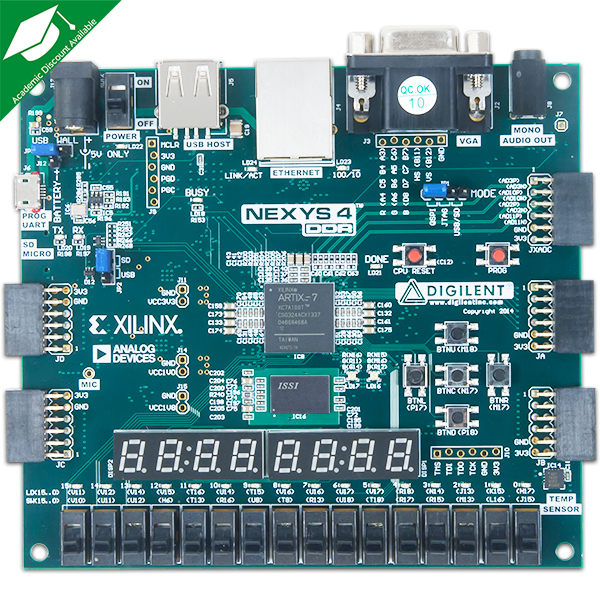
\includegraphics[width=0.75\linewidth]{nexys4ddr}
  \caption{The Nexys 4 DDR Artix-7 FPGA Trainer Board}
  \label{fig:nexys4ddr}
\end{figure}

\begin{figure}
  \centering
  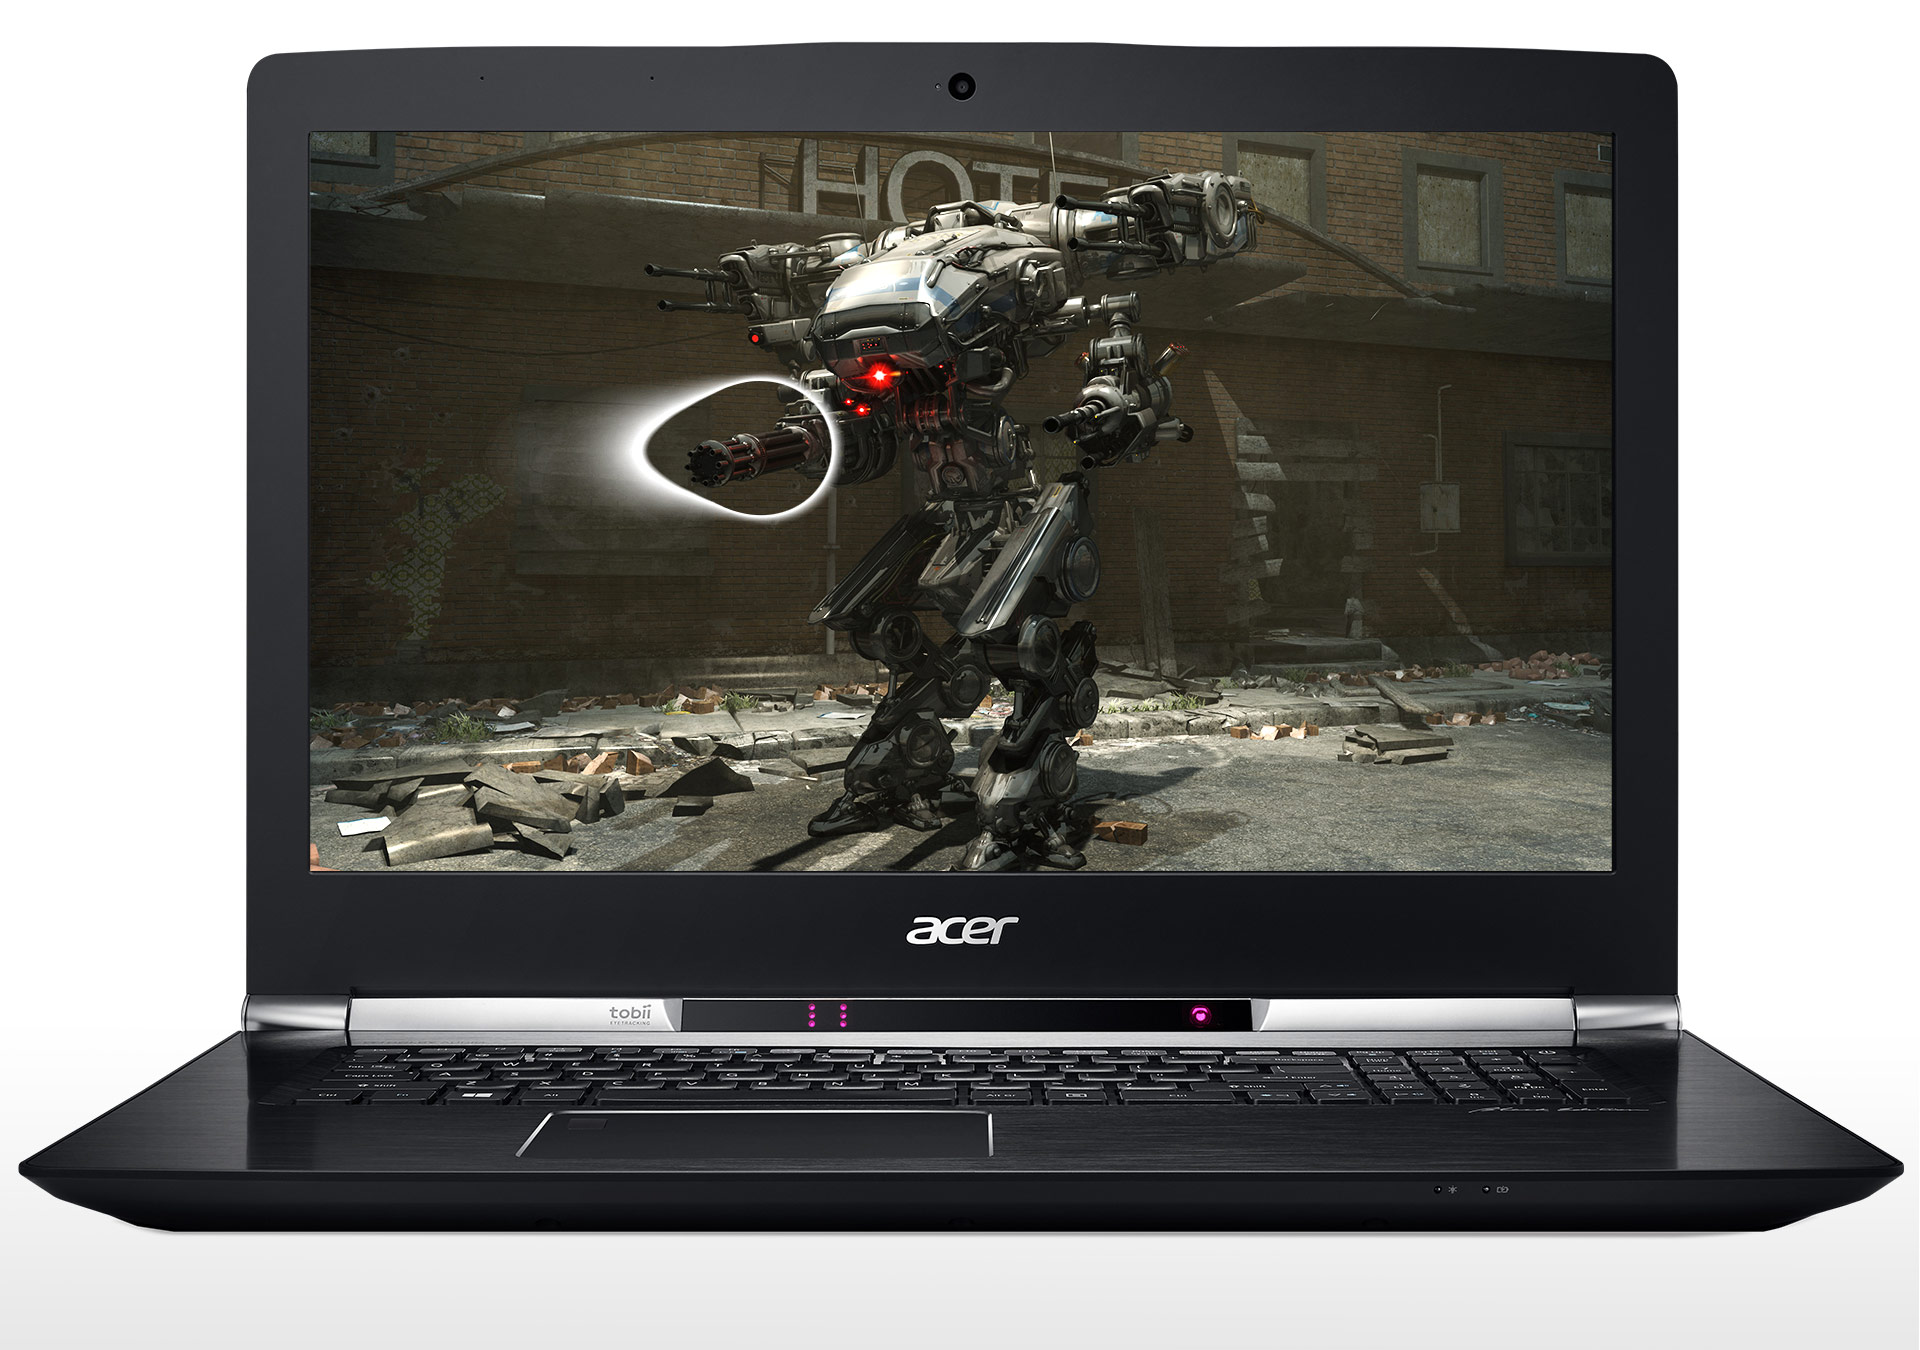
\includegraphics[width=0.75\linewidth]{aspirevnitro}
  \caption{The Acer Aspire V Nitro Laptop}
  \label{fig:aspirevnitro}
\end{figure}

%-----------------------------------
%	SUBSECTION 1
%-----------------------------------
\subsection{Software Used}

\label{Ch3 Sec2 Sub2}

During development of the MEGA65 several software packages were used in order to interact with the hardware listed above. These packages include:\\

\begin{itemize}
\item{Ubuntu 18.04: This operating system was required for work on the project. It was through it that commands required to program and interact with the FPGA were able to function.}
\item{Vivado HLx Webpack Edition: The development tools that this webpack provided was critical for the function of the MEGA65. These tools were used to program and make changes to the FPGA.}
\item{Git: This version control tool, while not necessary, was extremely useful. This allowed changes to be tracked and shared between developers on the project. The hosted repositories are found on the GitHub website}
\item{GHDL: This VHDL simulation software was very useful when debugging during the project. It allowed for more easily accessible variables during run time.}
\end{itemize}

% Chapter Template

\chapter{Project Set-up} % Main chapter title

\label{Chapter 4} % Change X to a consecutive number; for referencing this chapter elsewhere, use \ref{ChapterX}

This chapter describes the issues encountered prior to beginning the objectives stated in section \ref{Ch1 Sec2}. This section start by discussing why there were dependency issues experienced when starting the project. It then goes on to specifically identify the issues and the steps taken to correct these issues. Then, in section \ref{Ch4 Sec2}, the issues that were experienced with fdisk are highlighted and the solution discussed. 

%----------------------------------------------------------------------------------------
%	SECTION 1
%----------------------------------------------------------------------------------------

\section{Dependency Issues}

\label{Ch4 Sec1}

The MEGA65 project is an open source project, this works to the benefit, but also to the detriment of the project. Because there are many developers on the project, it is not well documented and the source code is prone to dependency issues that are only problems for newer developers. In addition to the the large developer base, the iterative development cycle and trial and error bug fixing has also caused dependency issues to be present in the source code.

%-----------------------------------
%	SUBSECTION 1
%-----------------------------------
\subsection{Missing Sub-Modules}

\label{Ch4 Sec1 Sub1}

During synthesis errors would often occur due to missing commands that were used in the makefile, but were not natively supported by Ubuntu Linux. The missing commands commands were the cc65 command, the ca65 command, the ld65 command, cbmconvert command and the ophis command. The cc65 command was used as the C compiler for the 6502 CPU. The ca65 was used in conjunction with the cc65 compiler as the assembler for the 6502 CPU. The ld65 was used as the linker to create an executable file from the object files. In addition to the missing compilation commands the cross-assembler, ophis, and the Commodore binary converter, cbmconvert, commands were not present in the project. These commands were developed separately from the MEGA65 and accessible through their own github repositories. This separation from the MEGA65 project caused each developer to reference the required commands differently, making the use of one universal makefile impossible. In order to correct this, as seen in figure \ref{fig:mega65MakerfileSubmodulesUpdates}, the source code for each required command was initialised as a sub-module of the project. This allowed the making of the project to automatically download, update and build the commands required later during synthesis.\\

\begin{figure}
  \centering
  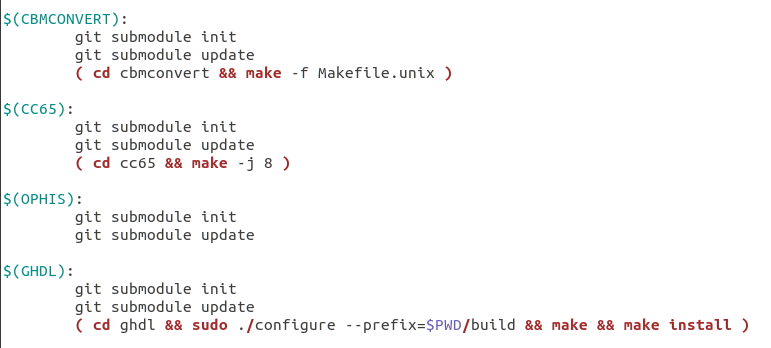
\includegraphics[width=\linewidth]{mega65MakerfileSubmoduleUpdates}
  \caption{The makefile with sub-module initialisation and make additions.}
  \label{fig:mega65MakerfileSubmodulesUpdates}
\end{figure}

Additionally, for these new sub-modules to be used, the pathing in the makefile was changed to correctly reference the required commands. Figure \ref{fig:mega65MakerfilePathing} shows that, thanks to sub-modules being located in the project directory, absolute pathing to the commands can now be done.\\

\begin{figure}
  \centering
  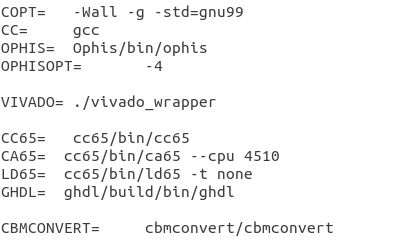
\includegraphics[width=\linewidth]{mega65MakerfilePathing}
  \caption{The updated referencing of the sub-modules}
  \label{fig:mega65MakerfilePathing}
\end{figure}

For the initialising and updating additions to the makefile to be useful, each instance where a sub-module is being used was updated to include a call to the sections seen in \ref{fig:mega65MakerfileSubmodulesUpdates}. One such example of these updates can be seen in figure \ref{fig:mega65AutoBuild}.\\

\begin{figure}
  \centering
  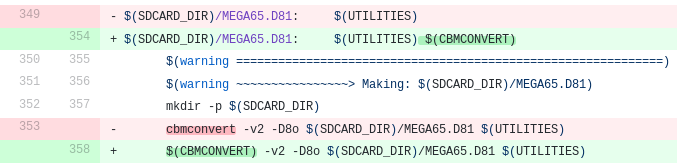
\includegraphics[width=\linewidth]{mega65AutoBuild}
  \caption{The updated function calls that reference the code seen in \ref{fig:mega65MakerfileSubmodulesUpdates}.}
  \label{fig:mega65AutoBuild}
\end{figure}

%----------------------------------------------------------------------------------------
%	SECTION 2
%----------------------------------------------------------------------------------------

\section{Fdisk}

\label{Ch4 Sec2}

In order to partition the MEGA65, the command line tool fdisk was created; this tool was already made a sub-module of the MEGA65 project. Similar to the MEGA65 source code, the fdisk source code had dependency issues in it due to it's open source nature. Specifically, due to the cc65 and cl65 commands being required and the unusuallity of fdisk tool being compiled separately from the MEGA65 project. The pathing for the cc65 and cl65 commands in the mega65-fdisk makefile was incorrect. As seen in figure \ref{fig:fdisk}, previously the cc65 and cl65 commands was just copied into the repository, which was not ideal as the fdisk repository was supposed to be able to be built independently from the rest of the mega65 project. Similar to section \ref{Ch4 Sec1}, the cc65 repository was made a sub-module of the fdisk repository and the fdisk makerfile was changed to automatically initialise it and build it while making fdisk. These changes are shown in figure \ref{fig:fdisk}.\\

\begin{figure}
  \centering
  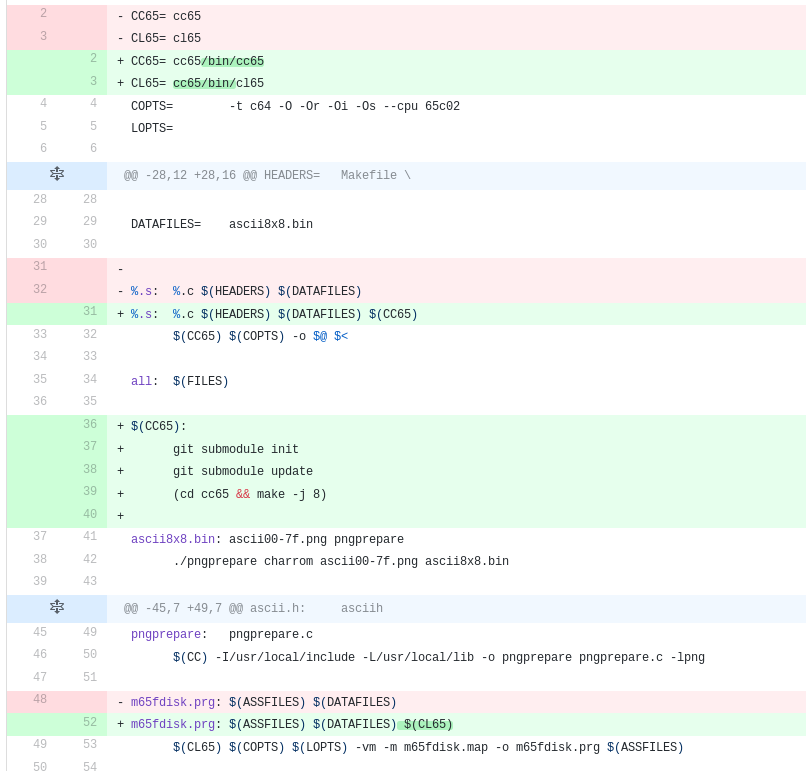
\includegraphics[width=\linewidth]{fdisk}
  \caption{fdisk sub-module dependency changes.}
  \label{fig:fdisk}
\end{figure}

 
% Chapter Template

\chapter{Matrix Mode Corrections} % Main chapter title

\label{Chapter 5} % Change X to a consecutive number; for referencing this chapter elsewhere, use \ref{ChapterX}

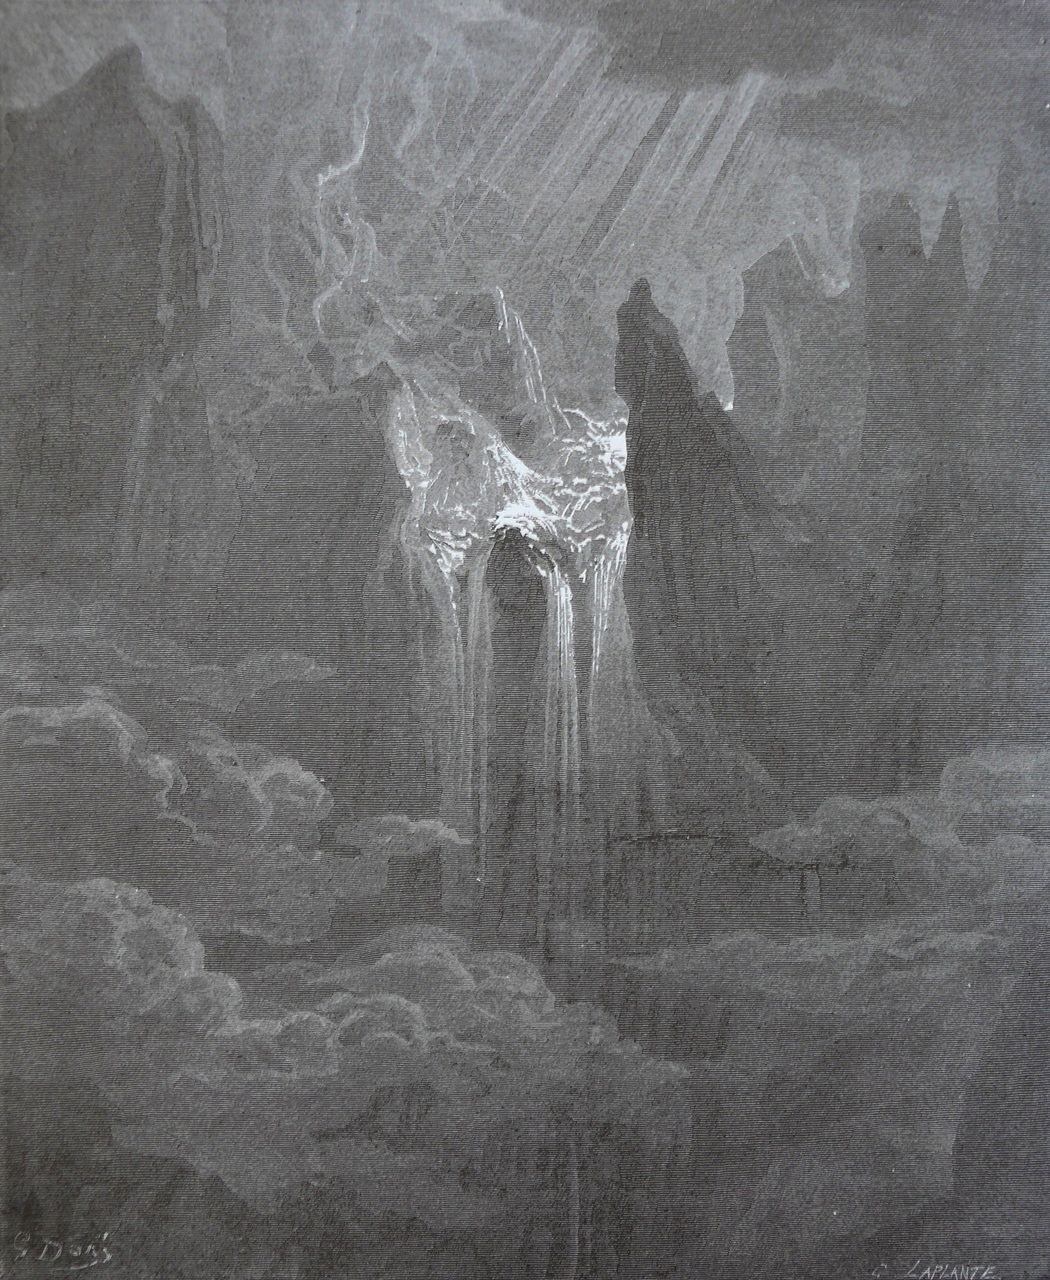
\includegraphics[width=\linewidth,trim={0 16cm 0 3cm},clip]{Paradise_Lost_30}

\section{Overview}

In the following chapter the issues discovered in matrix mode are outlined, analysed and then the solutions to the problems are described. This begins with the serial interface locking issue and then moves onto the uart monitor, matrix mode compositor handshaking issue. The letterboxing implementation is then discussed and the chapter is ended with the smaller bug fixes to matrix mode.

%----------------------------------------------------------------------------------------
%	SECTION 1
%----------------------------------------------------------------------------------------

\section{Serial Locking}

\label{Ch5 Sec1}

One existing issue with the phone was that when it entered matrix mode, the serial interface with the board would lock up. This would render all attempts at interfacing with the MEGA65 useless. Locking the serial input to the device was expected whilst in matrix mode, as this would prevent subversion of during sensitive program execution. The failure to return serial functionality to the device upon leaving matrix mode was showed that there was some handshaking protocols that were not behaving as expected.This phenomenon was especially strange as the code to disable the serial input while in matrix mode was removed for debug purposes. This proved that it was not entering or exiting matrix mode that caused the bug, but some protocol within the character processing or character displaying.

%-----------------------------------
%	SUBSECTION 1
%-----------------------------------
\subsection{Creating the Test-bench}

\label{Ch5 Sec1 Sub1}

Due to the long synthesis times, in excess of an hour, a light weight version of the phone needed to be created. Thanks to debugging in the past, this problem had already been encountered and solved. In order to save time during synthesis previously, a version of the phone was created without the CPU. This version was outdated and required some additional ports to spoof the components into working correctly. A CPU free version of the phone, some of which can be seen in figures \ref{fig:nocpuzero}, \ref{fig:nocpuone}, \ref{fig:nocputwo}, was possible thanks to matrix mode being composited over the video feed in hardware, rather than being done in software. Once the CPU free components were working, a Vivado technical command language (tcl) file was acquired from one of the other contributors to the project. This file was used to set up and execute the vivado tasks required to create and compile the CPU-less version of the phone. This resulted in a bit stream that was able to be run on the Nexys4ddr boards in the lab.

\begin{figure}
  \centering
  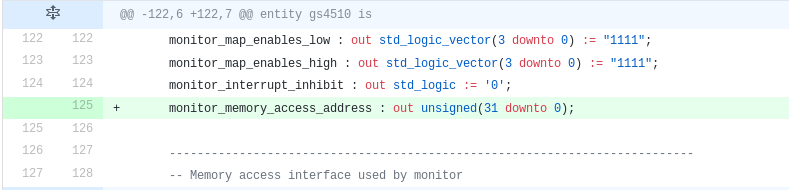
\includegraphics[width=\linewidth]{nocpuzero}
  \caption{Addition of monitor memory access address port to the nocpu.vhdl file.}
  \label{fig:nocpuzero}
\end{figure}

\begin{figure}
  \centering
  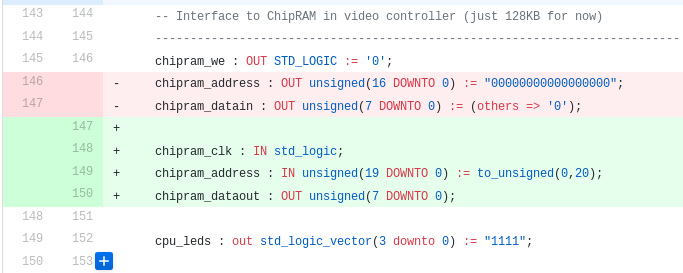
\includegraphics[width=\linewidth]{nocpuone}
  \caption{Addition of the chip ram clock and modification to the chip ram address and data ports in nocpu.vhdl.}
  \label{fig:nocpuone}
\end{figure}

\begin{figure}
  \centering
  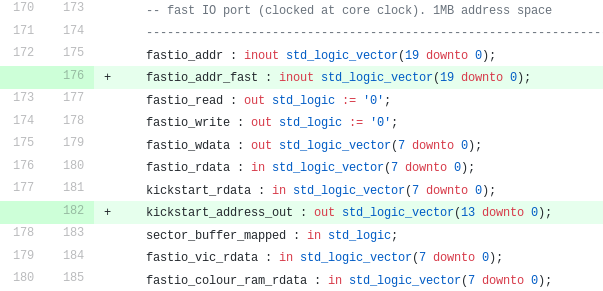
\includegraphics[width=\linewidth]{nocputwo}
  \caption{Fast I/O address port and kickstart address port additions to the nocpu.vhdl file.}
  \label{fig:nocputwo}
\end{figure}

%-----------------------------------
%	SUBSECTION 2
%-----------------------------------
\subsection{Timing Issues}

\label{Ch5 Sec1 Sub2}

One of the theorised causes for the serial locking issue was that the timing between the handshaking protocols was misaligned and was causing a state in which the serial output was not able to be read. In order to find these issues a timing report needed to be generated during synthesis. This was achieved by altering the tcl file and enabling the timing report generation, as seen in figure \ref{fig:timing}. This change was done to all of the tcl files as it would allow any type of synthesis, no CPU or otherwise, to generate timing reports. This would assist in identifying when signals that extend synthesis due to timing issues in the future. In the timing reports generated, several video signals were found to be causing timing issues; to solve these an intermediary signal was created to host the video data. As seen in figure \ref{fig:videodelay}, this would cause the data to be delayed by one clock cycle, the loss in time was determined to be acceptable as the difference of a pixel appearing a clock cycle late would not be perceptible to the human eye. This fix was not just applied to the vga signal, it was also applied to some signals in the frame generator, pixel mapper, io mapper and top level assembly. Some of the signals that were causing timing issues were unable to be driven, this was because they were determined to be critical. These signals required if statement reduction to reduce the logic delay between the source and destination registers. This was as the delay between the source and destination caused values in the outer statements to become stale before the inner logic could be resolved. In order to perform these reductions, the arguments in the inner statements were merged into the outer statements. Unfortunately, the resolution of the timing issues had no impact on the serial locking, but it did result in faster synthesis and a clearer image on the screen.

\begin{figure}
  \centering
  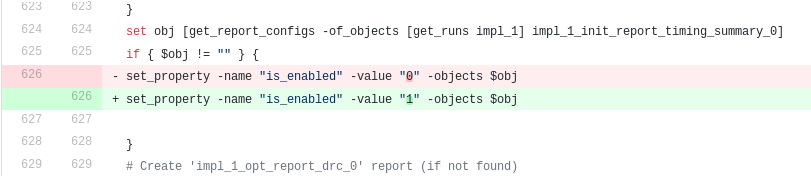
\includegraphics[width=\linewidth]{timing}
  \caption{The tcl file change that allowed the generation of timing reports.}
  \label{fig:timing}
\end{figure}

\begin{figure}
  \centering
  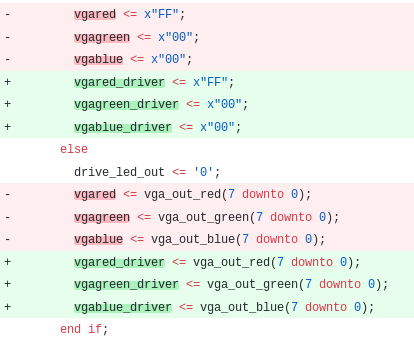
\includegraphics[width=\linewidth]{videodelay}
  \caption{Addition of vga driving signals to the viciv.vhdl file.}
  \label{fig:videodelay}
\end{figure}

%-----------------------------------
%	SUBSECTION 3
%-----------------------------------
\subsection{Handshaking Issues}

\label{Ch5 Sec1 Sub3}

As the timing issues were cleared, it was determined that the locking issue must be an error in the handshaking rather than a signal error. Firstly the keycode data that was passed from the terminal emulator to the rain compositor, as well as the iomapper key data and terminal emulator state were examined. This was done via the seven segment display on the nexys4ddr development board, as seen in figure \ref{fig:segleddata}. This revealed that the correct data was being passed prior to matrix mode and even after the lock had occurred. Further more, it showed that the terminal emulator was getting stuck in the print banner stage, in which, a predefined string was sent to the rain compositor. This suggested that the rest of the terminal emulator was working correctly and it was the output function that was causing the issue. Removing the printing section from the print banner state resulted in the serial output not locking up upon leaving matrix mode.\\

After further examining some of the flags associated with the output character function, it was noted that the terminal emulator would set two flags when sending characters, as seen in figure \ref{fig:outputchar}. The first is the character valid flag, it was observed to go high after a single character input and then never go low between subsequent inputs. This was also true for the second flag, the terminal emulator just sent flag. Looking for other instances of the both flags revealed that they were supposed to be reset while the terminal emulator was not ready, as seen in figure \ref{fig:termemureadyzero}. This terminal emulator ready flag was followed into the matrix rain compositor and it was discovered that the terminal emulator was only not ready when scrolling or when processing a character in the specific case seen in figure \ref{fig:termemureadytwo}. As these cases were correctly setting the terminal emulator to not ready when it was busy, the handshaking error was determined to be in the statement seen in figure \ref{fig:termemureadyzero}. Examining figure \ref{fig:termemureadyzero}, figure \ref{fig:termemureadytwo} and figure \ref{fig:outputchar} together, it can be seen that there is a logic clash when sending a character. The output character function sets the just sent and character valid flags high, which is then used to set the ready flag low, which is used to set the just sent and character valid flags low. This error was corrected by flipping the reset logic, as seen in figure \ref{fig:termemureadyone}. This resulted in matrix mode no longer locking up the serial input after processing a single character.

\begin{figure}
  \centering
  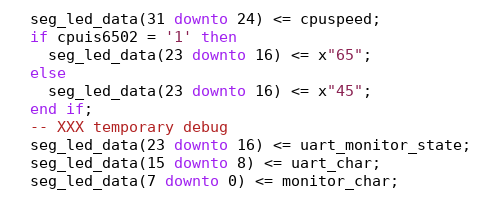
\includegraphics[width=\linewidth]{segleddata}
  \caption{Temporary debug output added to enable keyboard and serial keycode and terminal emulator state visualisation.}
  \label{fig:segleddata}
\end{figure}

\begin{figure}
  \centering
  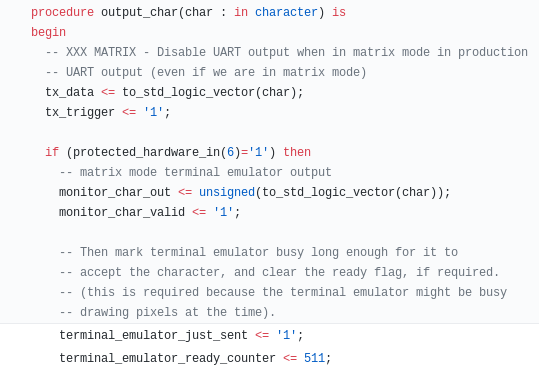
\includegraphics[width=\linewidth]{outputchar}
  \caption{The output character function within the uart monitor subsystem.}
  \label{fig:outputchar}
\end{figure}

\begin{figure}
  \centering
  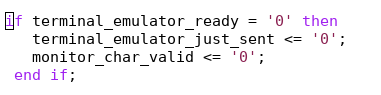
\includegraphics[width=\linewidth]{termemureadyzero}
  \caption{The monitor character valid and terminal emulator just sent flag reset statement.}
  \label{fig:termemureadyzero}
\end{figure}

\begin{figure}
  \centering
  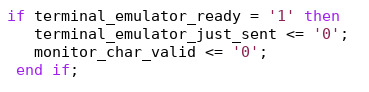
\includegraphics[width=\linewidth]{termemureadyone}
  \caption{The corrected monitor character valid and terminal emulator just sent flag reset statement.}
  \label{fig:termemureadyone}
\end{figure}

\begin{figure}
  \centering
  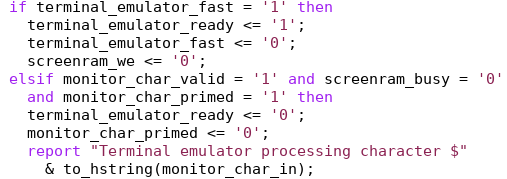
\includegraphics[width=\linewidth]{termemureadytwo}
  \caption{The matrix rain compositor character sequencing code.}
  \label{fig:termemureadytwo}
\end{figure}

%----------------------------------------------------------------------------------------
%	SECTION 2
%----------------------------------------------------------------------------------------

\section{Letterboxing}

\label{Ch5 Sec2}

One of the issues with matrix mode was that the matrix mode overlay was exceeding the desired bounds. This resulted in junk data to be loaded into the areas of the screen that were supposed to be blank. It also caused the top of the matrix mode display to appear above the visible portion of the screen and the end of matrix mode the continue off the screen, all of which can be seen in figure \ref{fig:noletterbox}.

%-----------------------------------
%	SUBSECTION 1
%-----------------------------------

\subsection{Makefile Correction}

\label{Ch5 Sec2 Sub1}

When looking at the error it was believed the the junk data was caused by rouge input from somewhere, as this input was always the same, it was determined to be some predefined string. Through an examination of matrix mode, it was discovered that the only source of input to the mode was the terminal emulator. Disconnecting the terminal emulator from the matrix rain compositor did not have any effect on the junk data being displayed however. This confirmed that the issue was not with the input to matrix mode, but in the compositor itself. Following the input characters into the matrix mode compositor lead to the case statement that handles the character processing and in particular, the case seen in figure \ref{fig:mmcharacterhandeling}. The monitor character can be seen being assigned to the screen ram write data, this write data signal is then used to write to the terminal memory, as seen in figure \ref{fig:mmscreenram}. This terminal memory, as seen by the use of screenram\_rdata in figure \ref{fig:mmtermmemout}, is then used to load character bits, which are then used to output characters to the screen. A joint examination of the terminal memory file with Dr. Gardner-Stephen, revealed that there were many preinitilized values in it via hardware. This was done in the makefile and the loaded values were the ASCII font and the matrix banner text. Removing both these from the terminal memory resolved the issue, but also resulted in no characters being able to be displayed. Further examination of the character set by Dr. Gardner-Stephen showed that two copies of it were being loaded into the terminal emulator and that one character set only required memory from location \$000 to location \$500. In order to remove this second character set from the terminal memory, after the character set was loaded, zeros were loaded into the address locations from \$800 to \$4095. This change, as seen in figure \ref{fig:termmemzeroing}, resulted in the matrix compositor only displaying unwanted characters in the lower portion of the screen. Figure \ref{fig:noletterboxromcorrection} shows change in issue, the remaining junk characters are either from the character set itself or the banner, both of which are unable to be removed from the terminal memory.

\begin{figure}
  \centering
  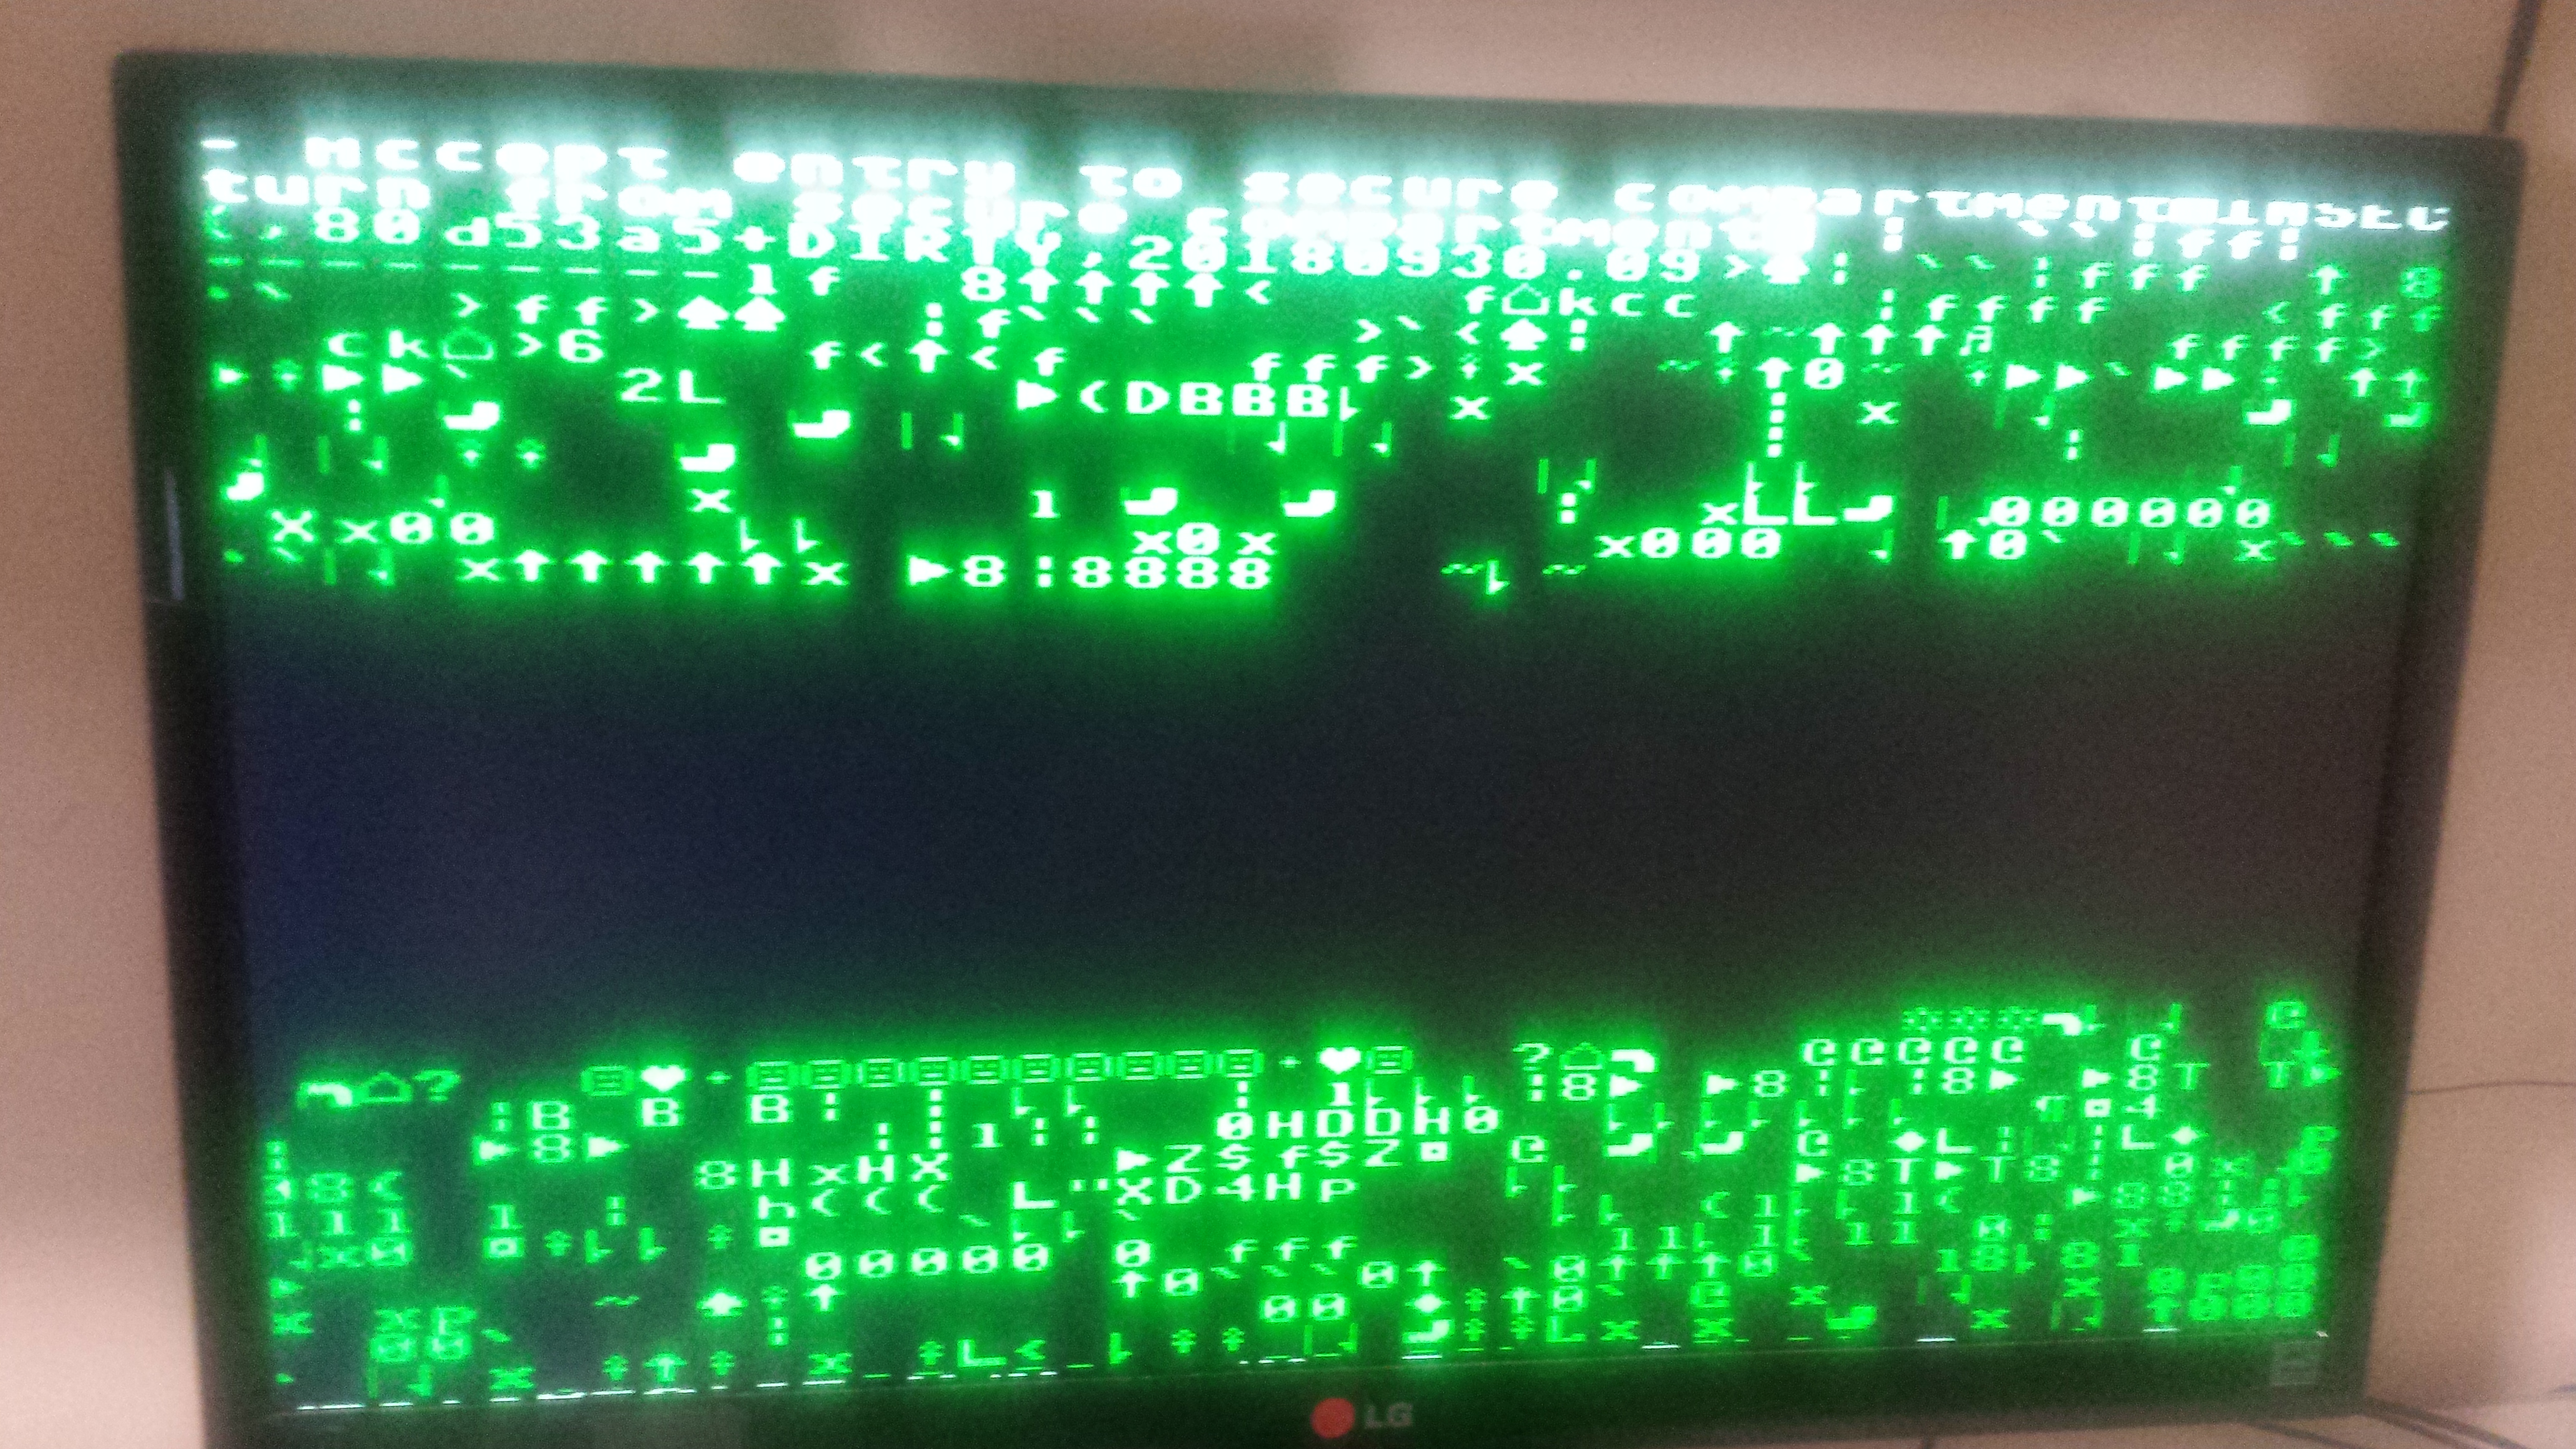
\includegraphics[width=\linewidth]{noletterbox}
  \caption{Matrix mode prior to letterbox fixes.}
  \label{fig:noletterbox}
\end{figure}

\begin{figure}
  \centering
  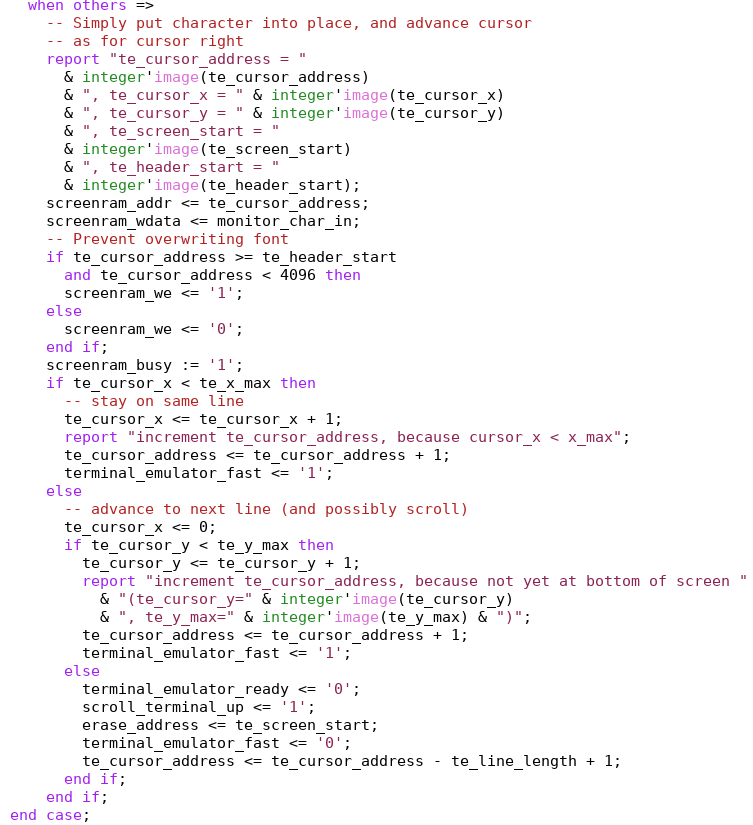
\includegraphics[width=\linewidth]{mmcharacterhandeling}
  \caption{The matrix rain compositor character processing code.}
  \label{fig:mmcharacterhandeling}
\end{figure}

\begin{figure}
  \centering
  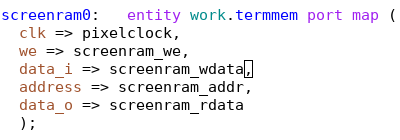
\includegraphics[width=\linewidth]{mmscreenram}
  \caption{The matrix mode screen ram entity.}
  \label{fig:mmscreenram}
\end{figure}

\begin{figure}
  \centering
  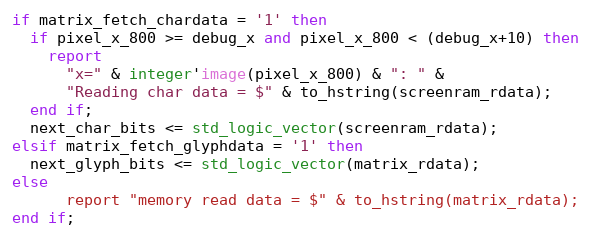
\includegraphics[width=\linewidth]{mmtermmemout}
  \caption{The assignment of the character bits in the terminal memory to the output variable.}
  \label{fig:mmtermmemout}
\end{figure}

\begin{figure}
  \centering
  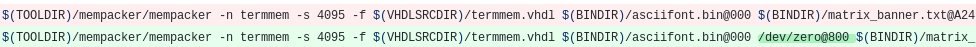
\includegraphics[width=\linewidth]{termmemzeroing}
  \caption{The makefile change to remove the excess character set from the terminal memory.}
  \label{fig:termmemzeroing}
\end{figure}

\begin{figure}
  \centering
  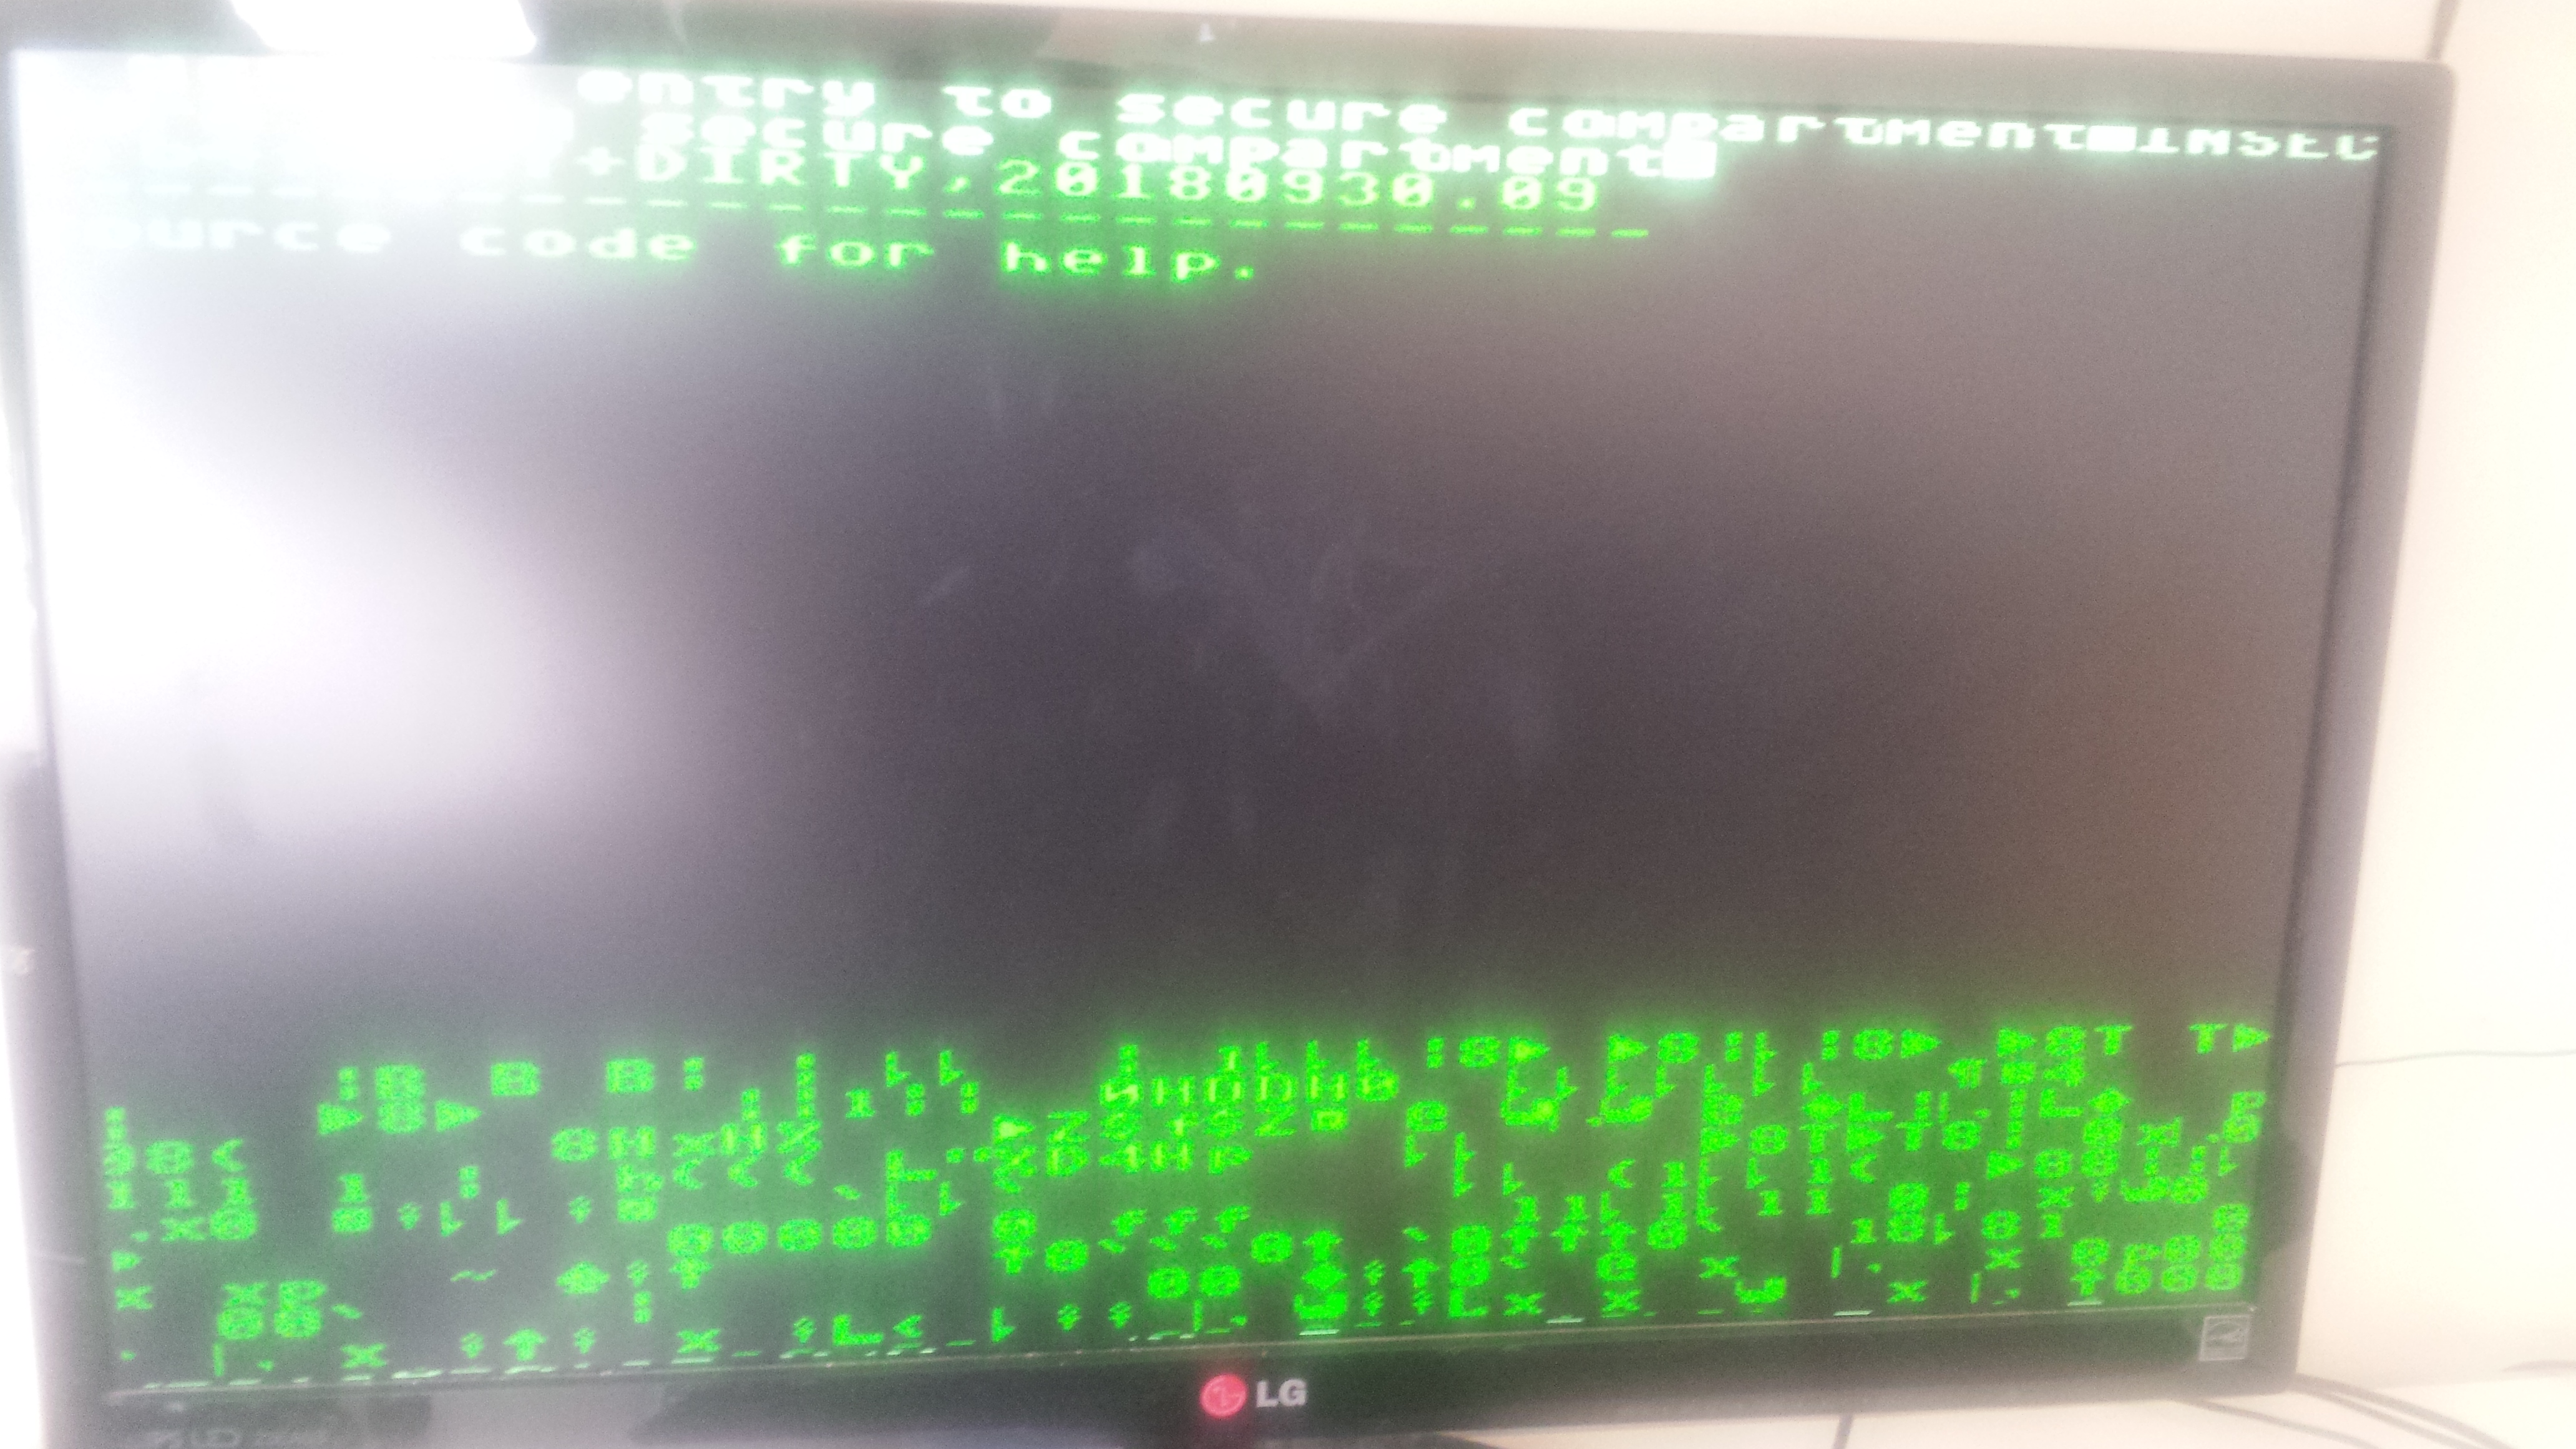
\includegraphics[width=\linewidth]{noletterboxromcorrection}
  \caption{Matrix mode without the second character set loaded into memory during compilation.}
  \label{fig:noletterboxromcorrection}
\end{figure}

%-----------------------------------
%	SUBSECTION 2
%-----------------------------------

\subsection{Letterbox Implementation}

\label{Ch5 Sec2 Sub2}

As the matrix mode display was still exceeding the desired bounds, a limiting signal was used to keep the visible output within a letterbox. One such signal already existed in the viciv and was being used for a similar purpose with the vga output. This signal was taken from the viciv and sent to the matrix mode compositor, where it was used in place of vsync. As seen in figure \ref{fig:letterboxcode}, in addition to the replacement of vsync, the letterbox signal was used to blank the region outside of the letterbox, this can be seen in figure \ref{fig:letterbox}. While the letterbox fixed the issues, it introduced some more minor issues into matrix mode. These issues are further discussed in the following sections.

\begin{figure}
  \centering
  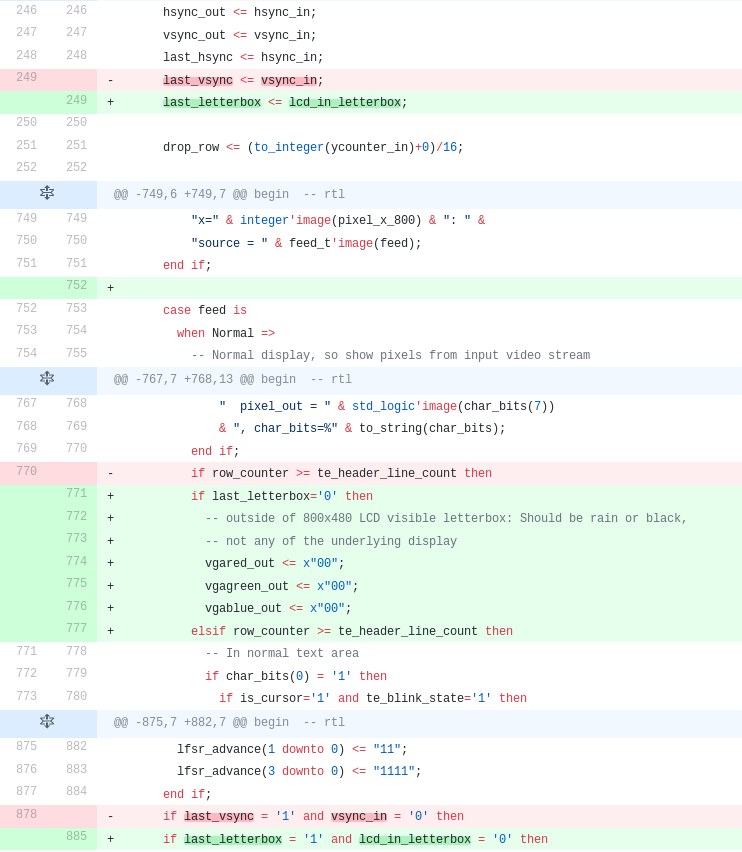
\includegraphics[width=\linewidth]{letterboxcode}
  \caption{The changes made to the matrix mode compositor to implement the letterboxing signal.}
  \label{fig:letterboxcode}
\end{figure}

\begin{figure}
  \centering
  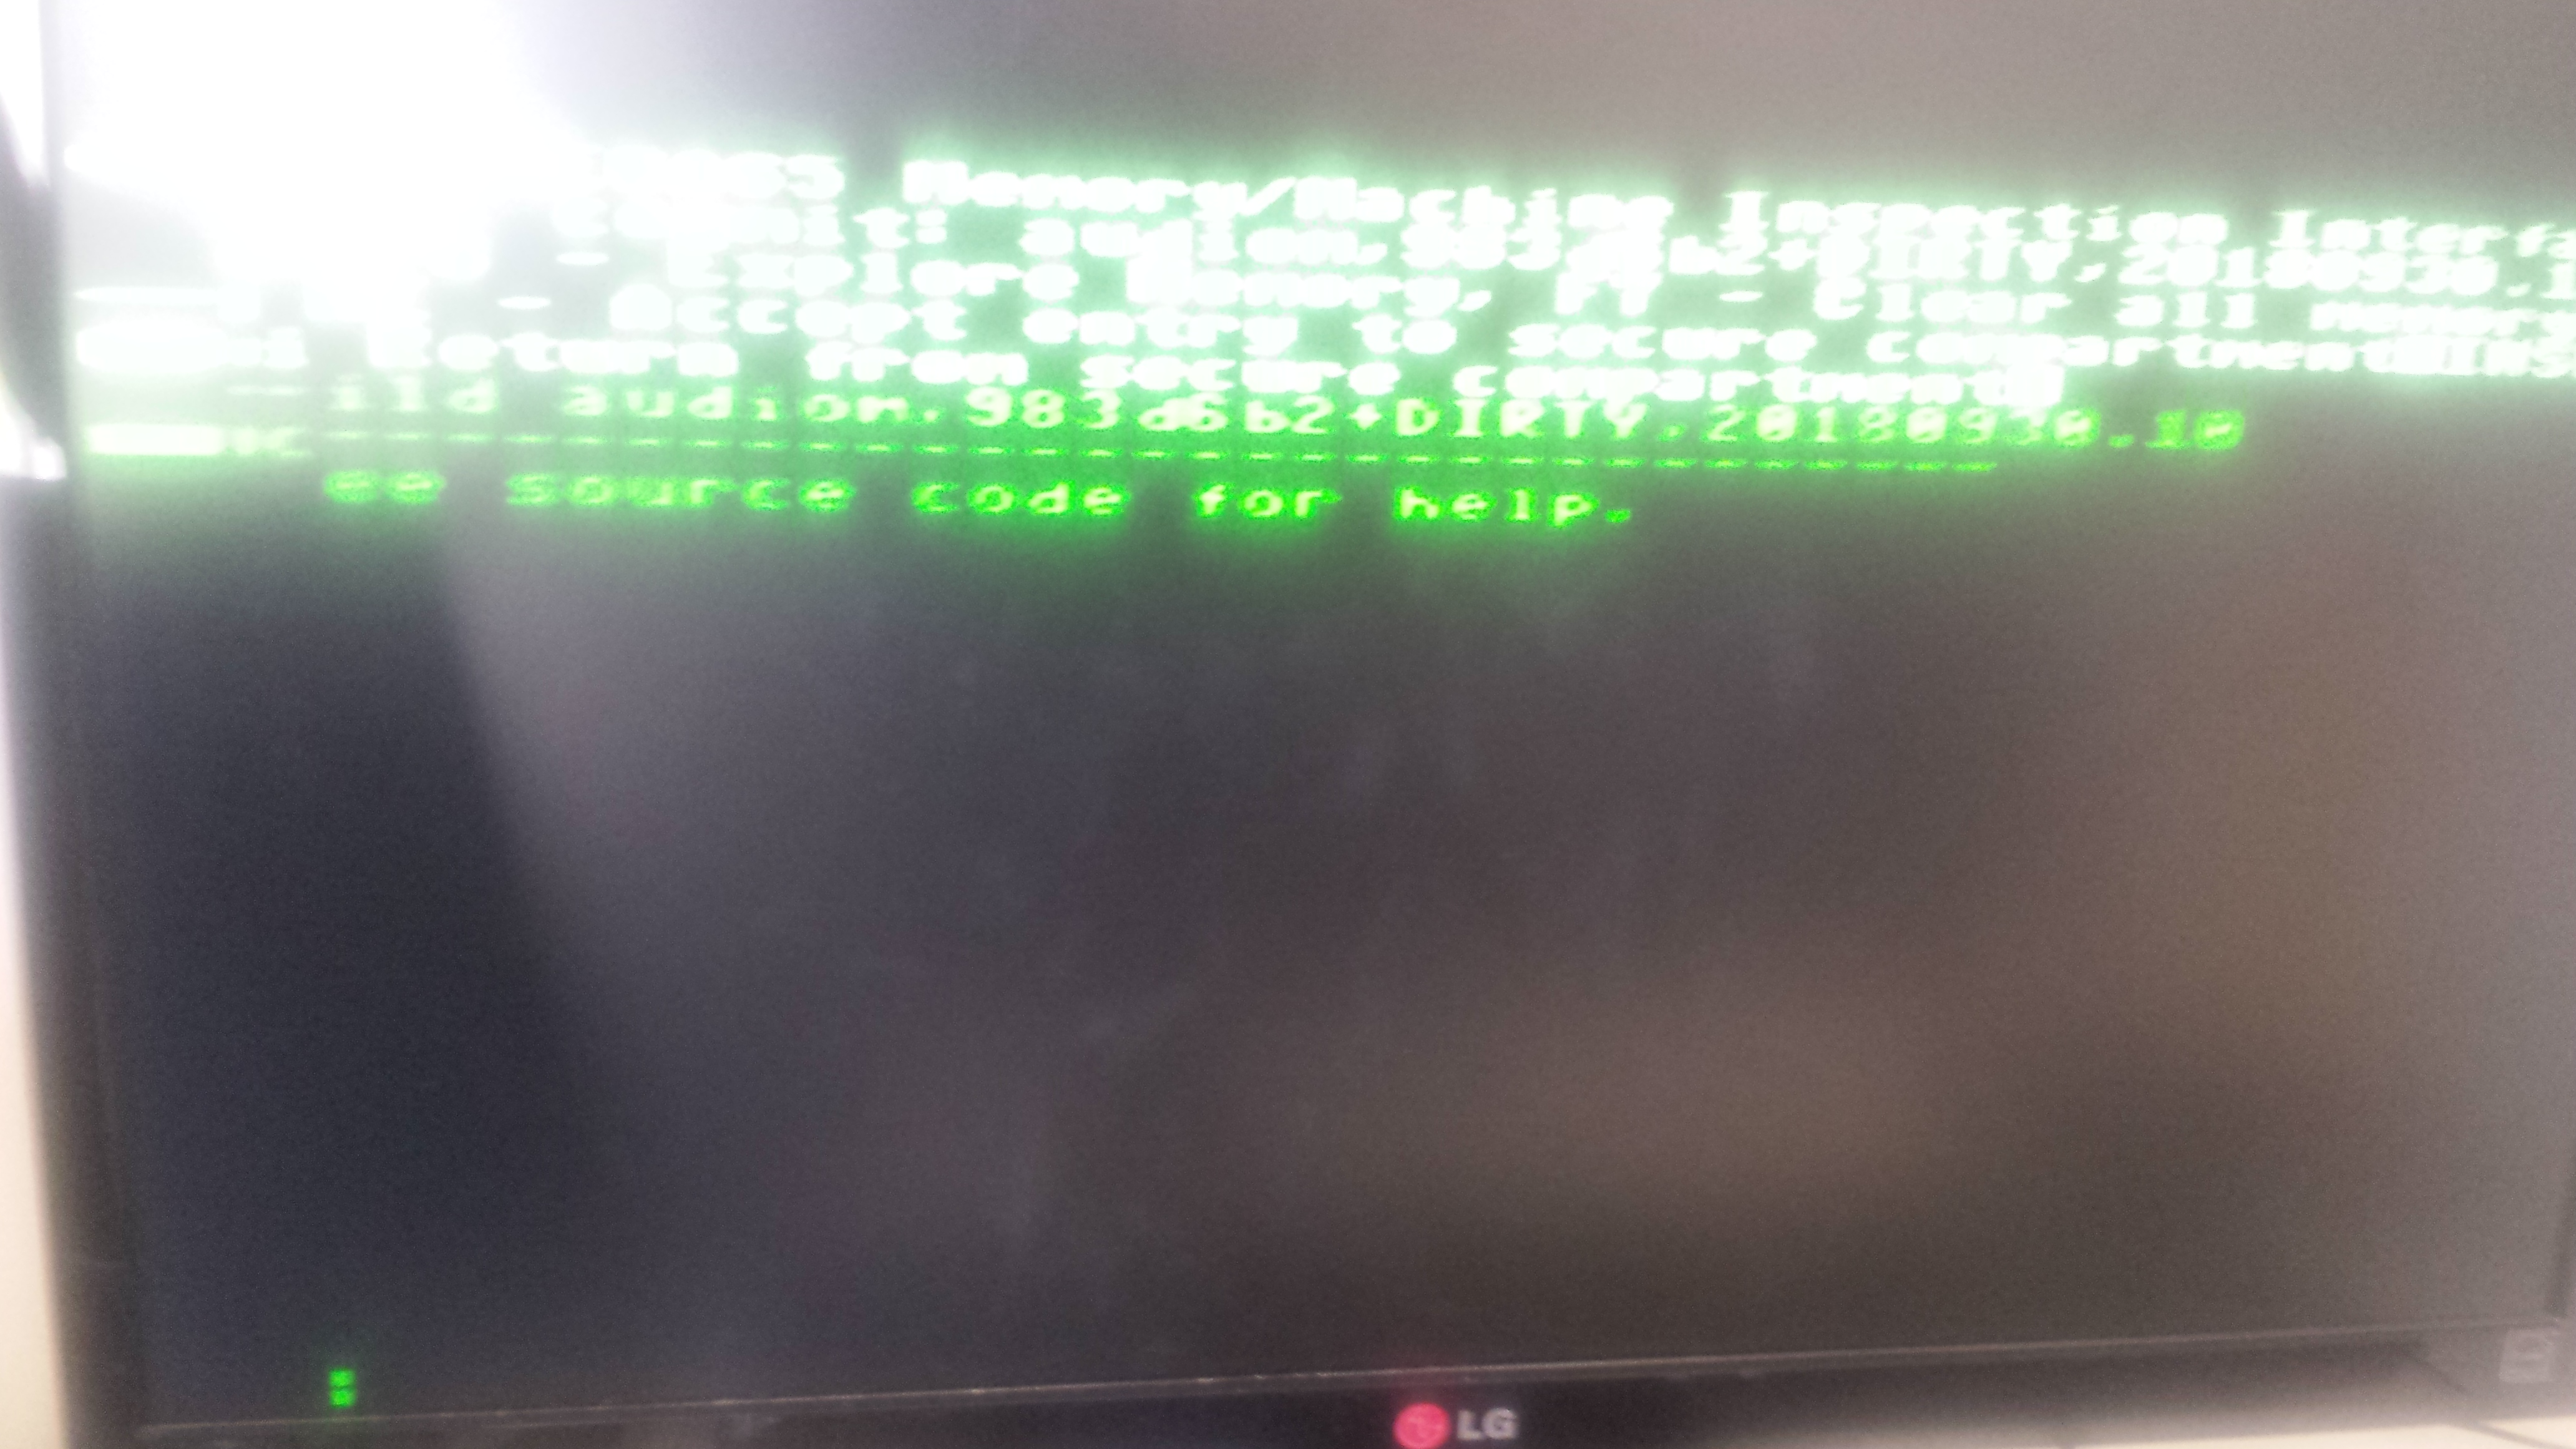
\includegraphics[width=\linewidth]{letterbox}
  \caption{Matrix mode with the letterboxing signal.}
  \label{fig:letterbox}
\end{figure}

%----------------------------------------------------------------------------------------
%	SECTION 4
%----------------------------------------------------------------------------------------

\section{Bug Fixing}

\label{Ch5 Sec3}

In addition to the matrix mode breaking bugs solved in sections \ref{Ch5 Sec1} and \ref{Ch5 Sec2}, there were also less urgent bugs in matrix mode that were solved. These bugs were graphical in nature and fixing them did not affect the overall functionality of matrix mode.

%-----------------------------------
%	SUBSECTION 1
%-----------------------------------

\subsection{Revolving Line}

\label{Ch5 Sec3 Sub1}

While restoring functionality to matrix mode it was noted that the input was not behaving as expected. A seen in figure \ref{fig:matrixmodelineinputerror}, whenever the cursor would go to a new line while scrolling it would move left one horizontal space. This resulted in the line revolving around the screen, this is believed to be due to under-flowing the horizontal position variable. Further examination of the variable, as seen in figure \ref{fig:revolvinglinezero} and figure \ref{fig:revolvinglineone}, show that during the new line handling while scrolling the cursor position is just rolled back to the start of the line. This does not take into account the full-stop used as an indication character at the start of each new line. The correction, as seen in figure \ref{fig:scrollline}, addresses this issue by starting the scrolled cursor position one increment to the right of the start of the line.

\begin{figure}
  \centering
  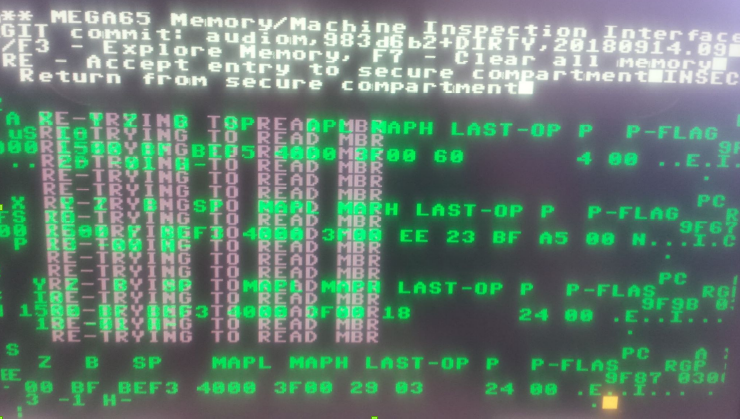
\includegraphics[width=\linewidth]{matrixmodelineinputerror}
  \caption{The matrix mode line revolution error.}
  \label{fig:matrixmodelineinputerror}
\end{figure}

\begin{figure}
  \centering
  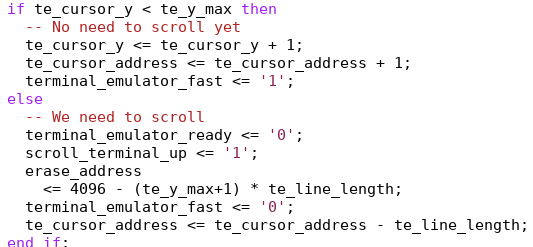
\includegraphics[width=\linewidth]{revolvinglinezero}
  \caption{The code used to handle the cursor address when scrolling in matrix mode.}
  \label{fig:revolvinglinezero}
\end{figure}

\begin{figure}
  \centering
  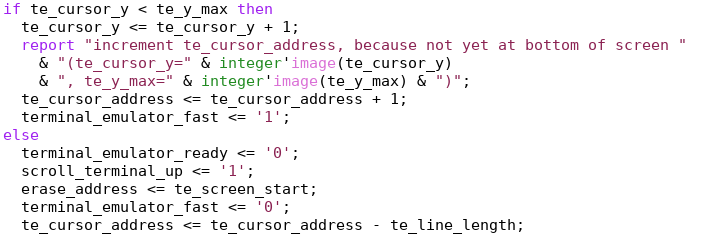
\includegraphics[width=\linewidth]{revolvinglineone}
  \caption{The code used when characters overflow onto the next line and scrolling is required.}
  \label{fig:revolvinglineone}
\end{figure}

\begin{figure}
  \centering
  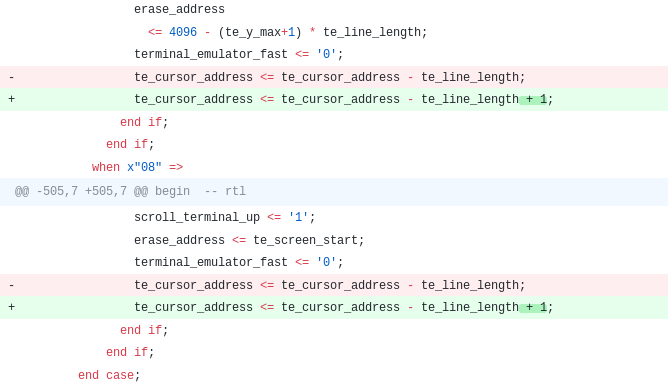
\includegraphics[width=\linewidth]{scrollline}
  \caption{The matrix rain compositor changes to eliminate the revolving line.}
  \label{fig:scrollline}
\end{figure}

%-----------------------------------
%	SUBSECTION 2
%-----------------------------------

\subsection{Bell Issue}

\label{Ch5 Sec3 Sub2}

During experimentation with the input to matrix mode it was noted that a strange character was being printed whenever the buffer overflowed. As identified by Dr. Gardner-Stephen, this character was intended to be the non printable bell character that would alert the user to an illegal action. This character can be seen as the "plus" symbols in figure \ref{fig:bellcharacter}. Examining the character output to the matrix mode compositor during when these bell characters were being output revealed that the key code being output was x"07". At the suggestion of Dr. Gardner-Stephen, an examination of the available keycodes showed that there was no case for this particular keycode. In order to stop this character from being printed, a case was added to handle it, as seen in figure \ref{fig:ignorebell}. This case would do nothing when it detected the bell character, this allowed for the character to be used later, while also preventing it from being printed. This introduced another error however, whenever a bell character was recognised it would lock up the input to matrix mode. This was due to the terminal emulator never being ready. Examination of the other cases showed that they all set terminal\_emulator\_fast to high after they had performed their case specific action. Implementing this, as seen in figure \ref{fig:newbell}, in the new case statement resulted in the issue being resolved.

\begin{figure}
  \centering
  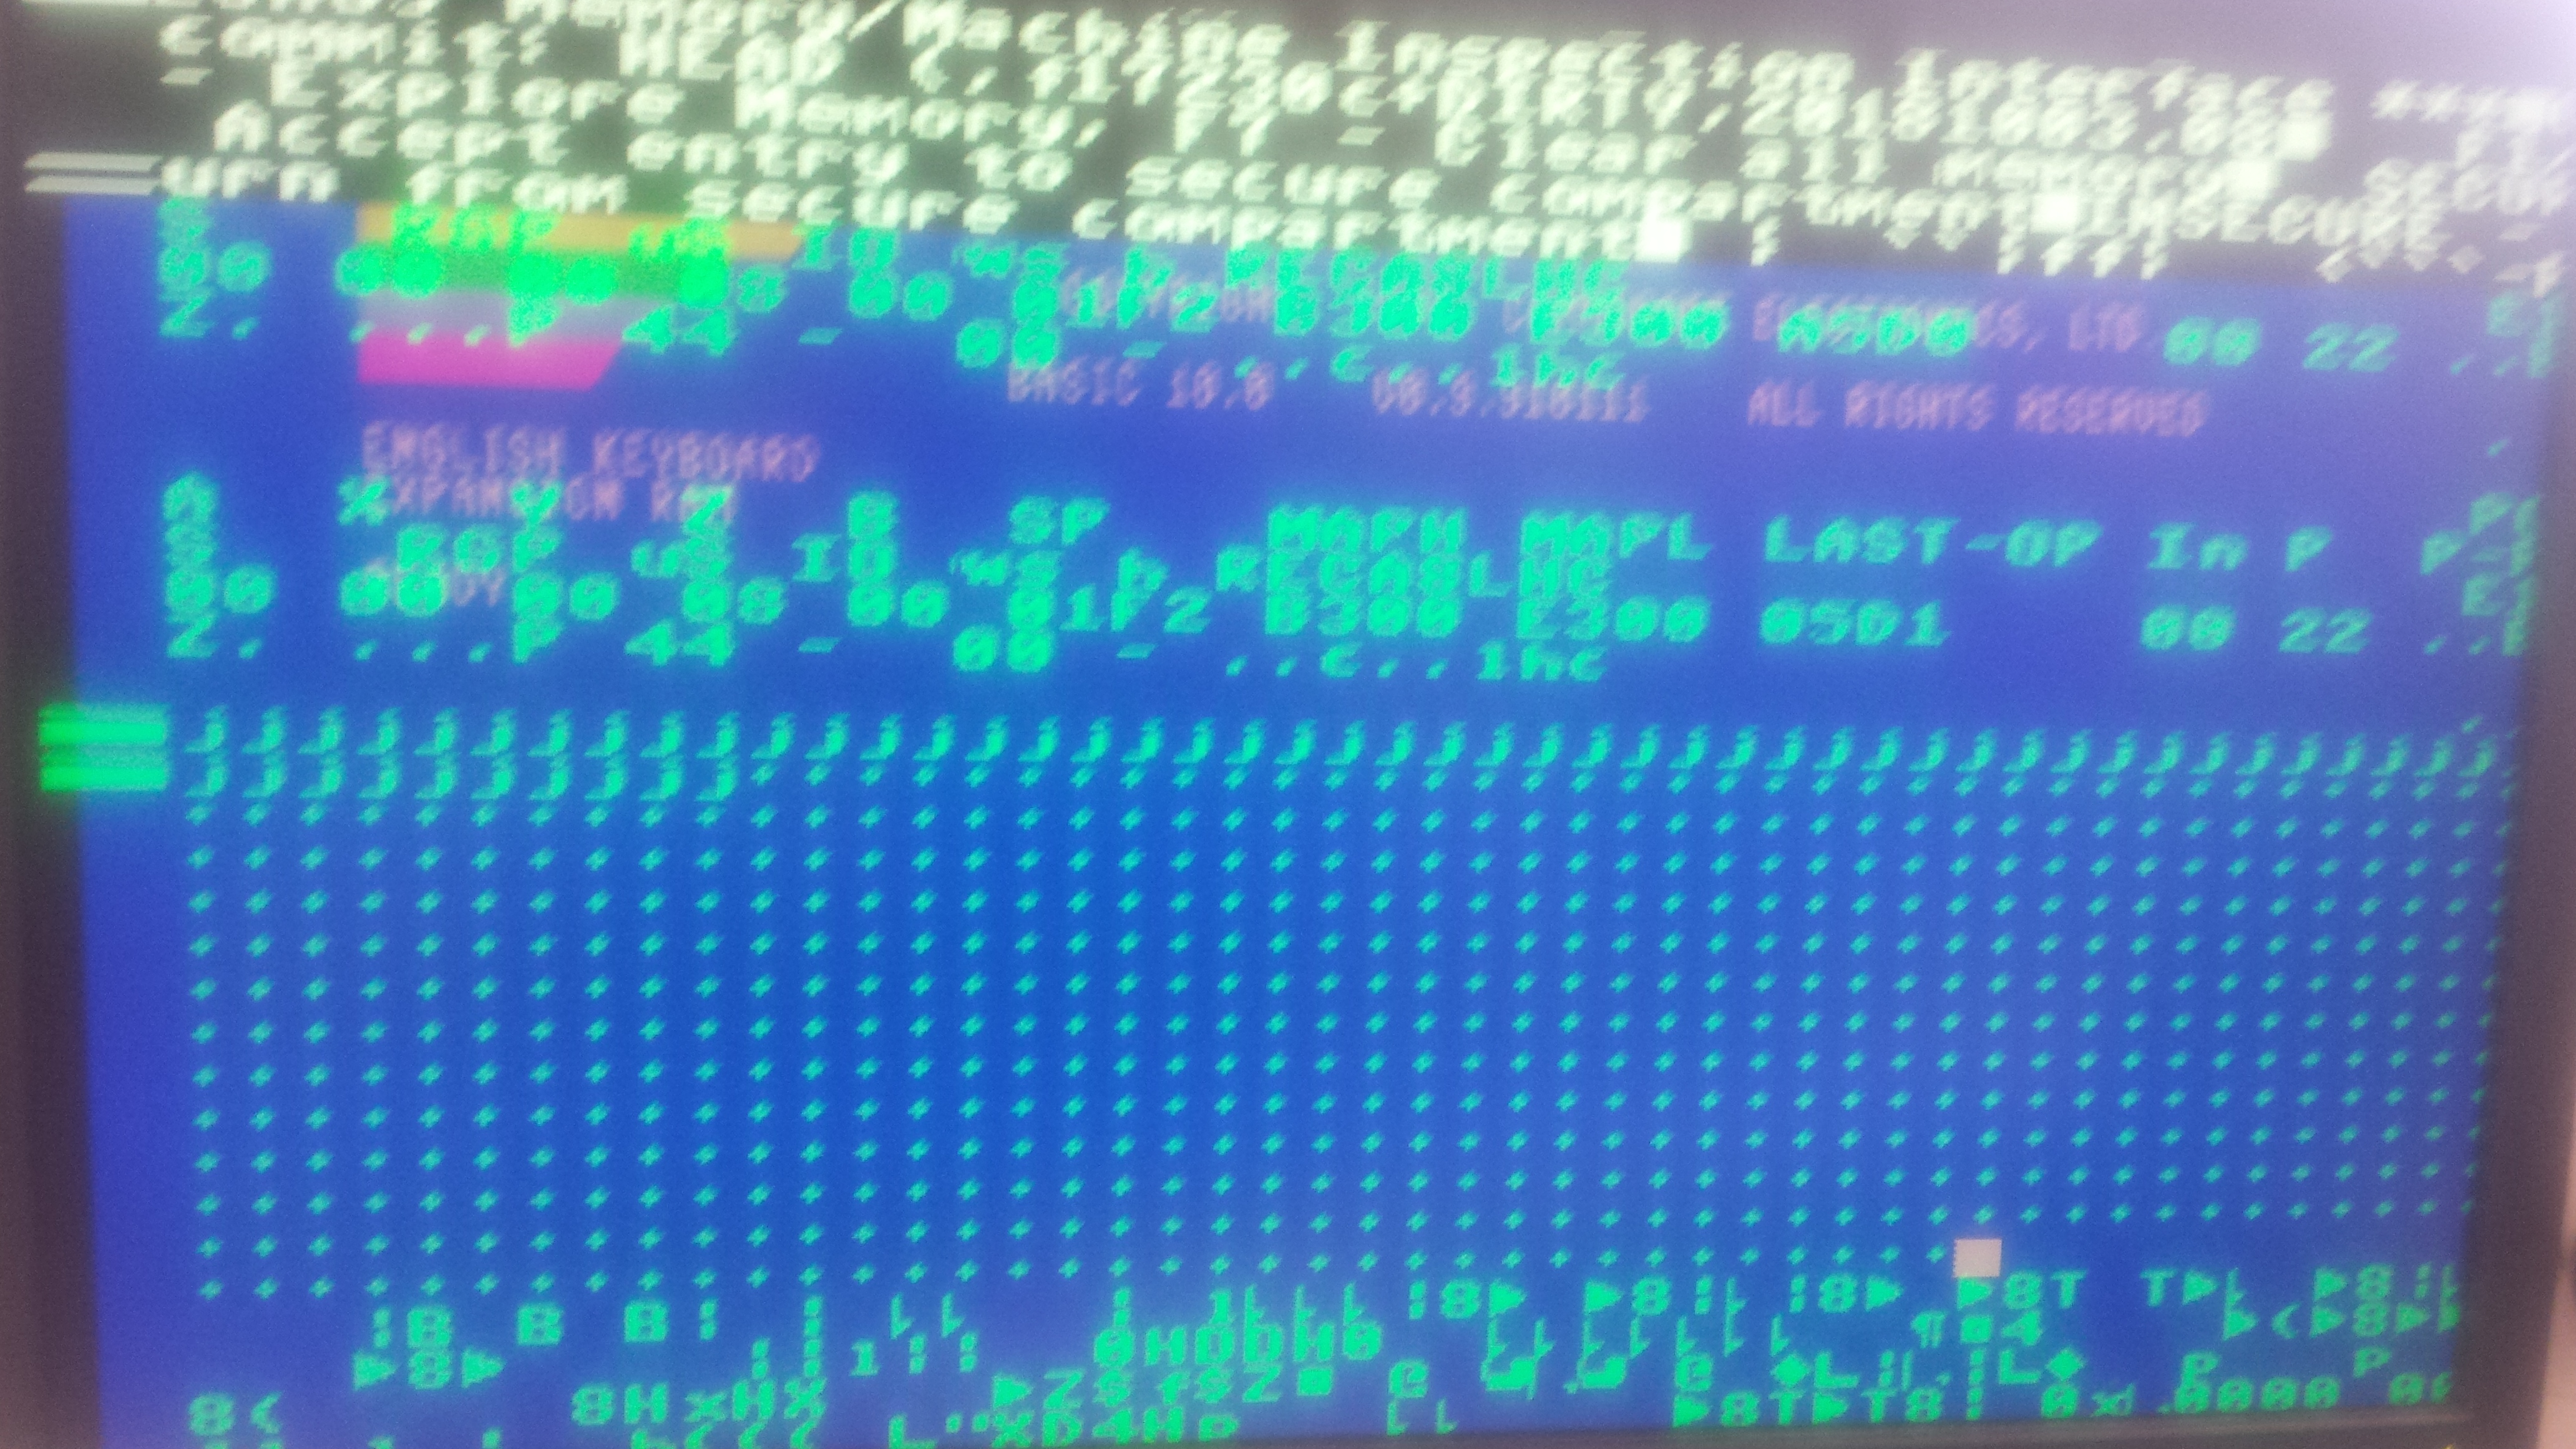
\includegraphics[width=\linewidth]{bellcharacter}
  \caption{The matrix mode with printed bell characters.}
  \label{fig:bellcharacter}
\end{figure}

\begin{figure}
  \centering
  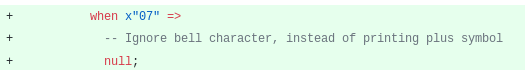
\includegraphics[width=\linewidth]{ignorebell}
  \caption{The case statement to ignore bell characters.}
  \label{fig:ignorebell}
\end{figure}

\begin{figure}
  \centering
  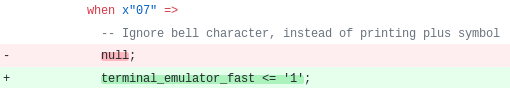
\includegraphics[width=\linewidth]{newbell}
  \caption{The change to the case statement to prevent serial locking.}
  \label{fig:newbell}
\end{figure}

%-----------------------------------
%	SUBSECTION 3
%-----------------------------------

\subsection{Pixel Shift}

\label{Ch5 Sec3 Sub3}

When examining the characters displayed to the screen, as noted in figure \ref{fig:biterror}, it was noted that some of them had their right most pixels wrapped around to the very left of the of the character tile. This output, as seen in figure \ref{fig:charbitstwo}, is due to the char\_bits variable. Tracing this variable back to its source revealed, as seen in figure \ref{fig:charbits}, that the bits for each character were being rotated around and used to decide whether to display a pixel or not. Dr. Garner-Stephen suggested, as the issue was a horizontal rotation, a rotation of the character bits should be performed, as displayed in figure \ref{fig:bitfix}. This fixed the pixel shift issue.

\begin{figure}
  \centering
  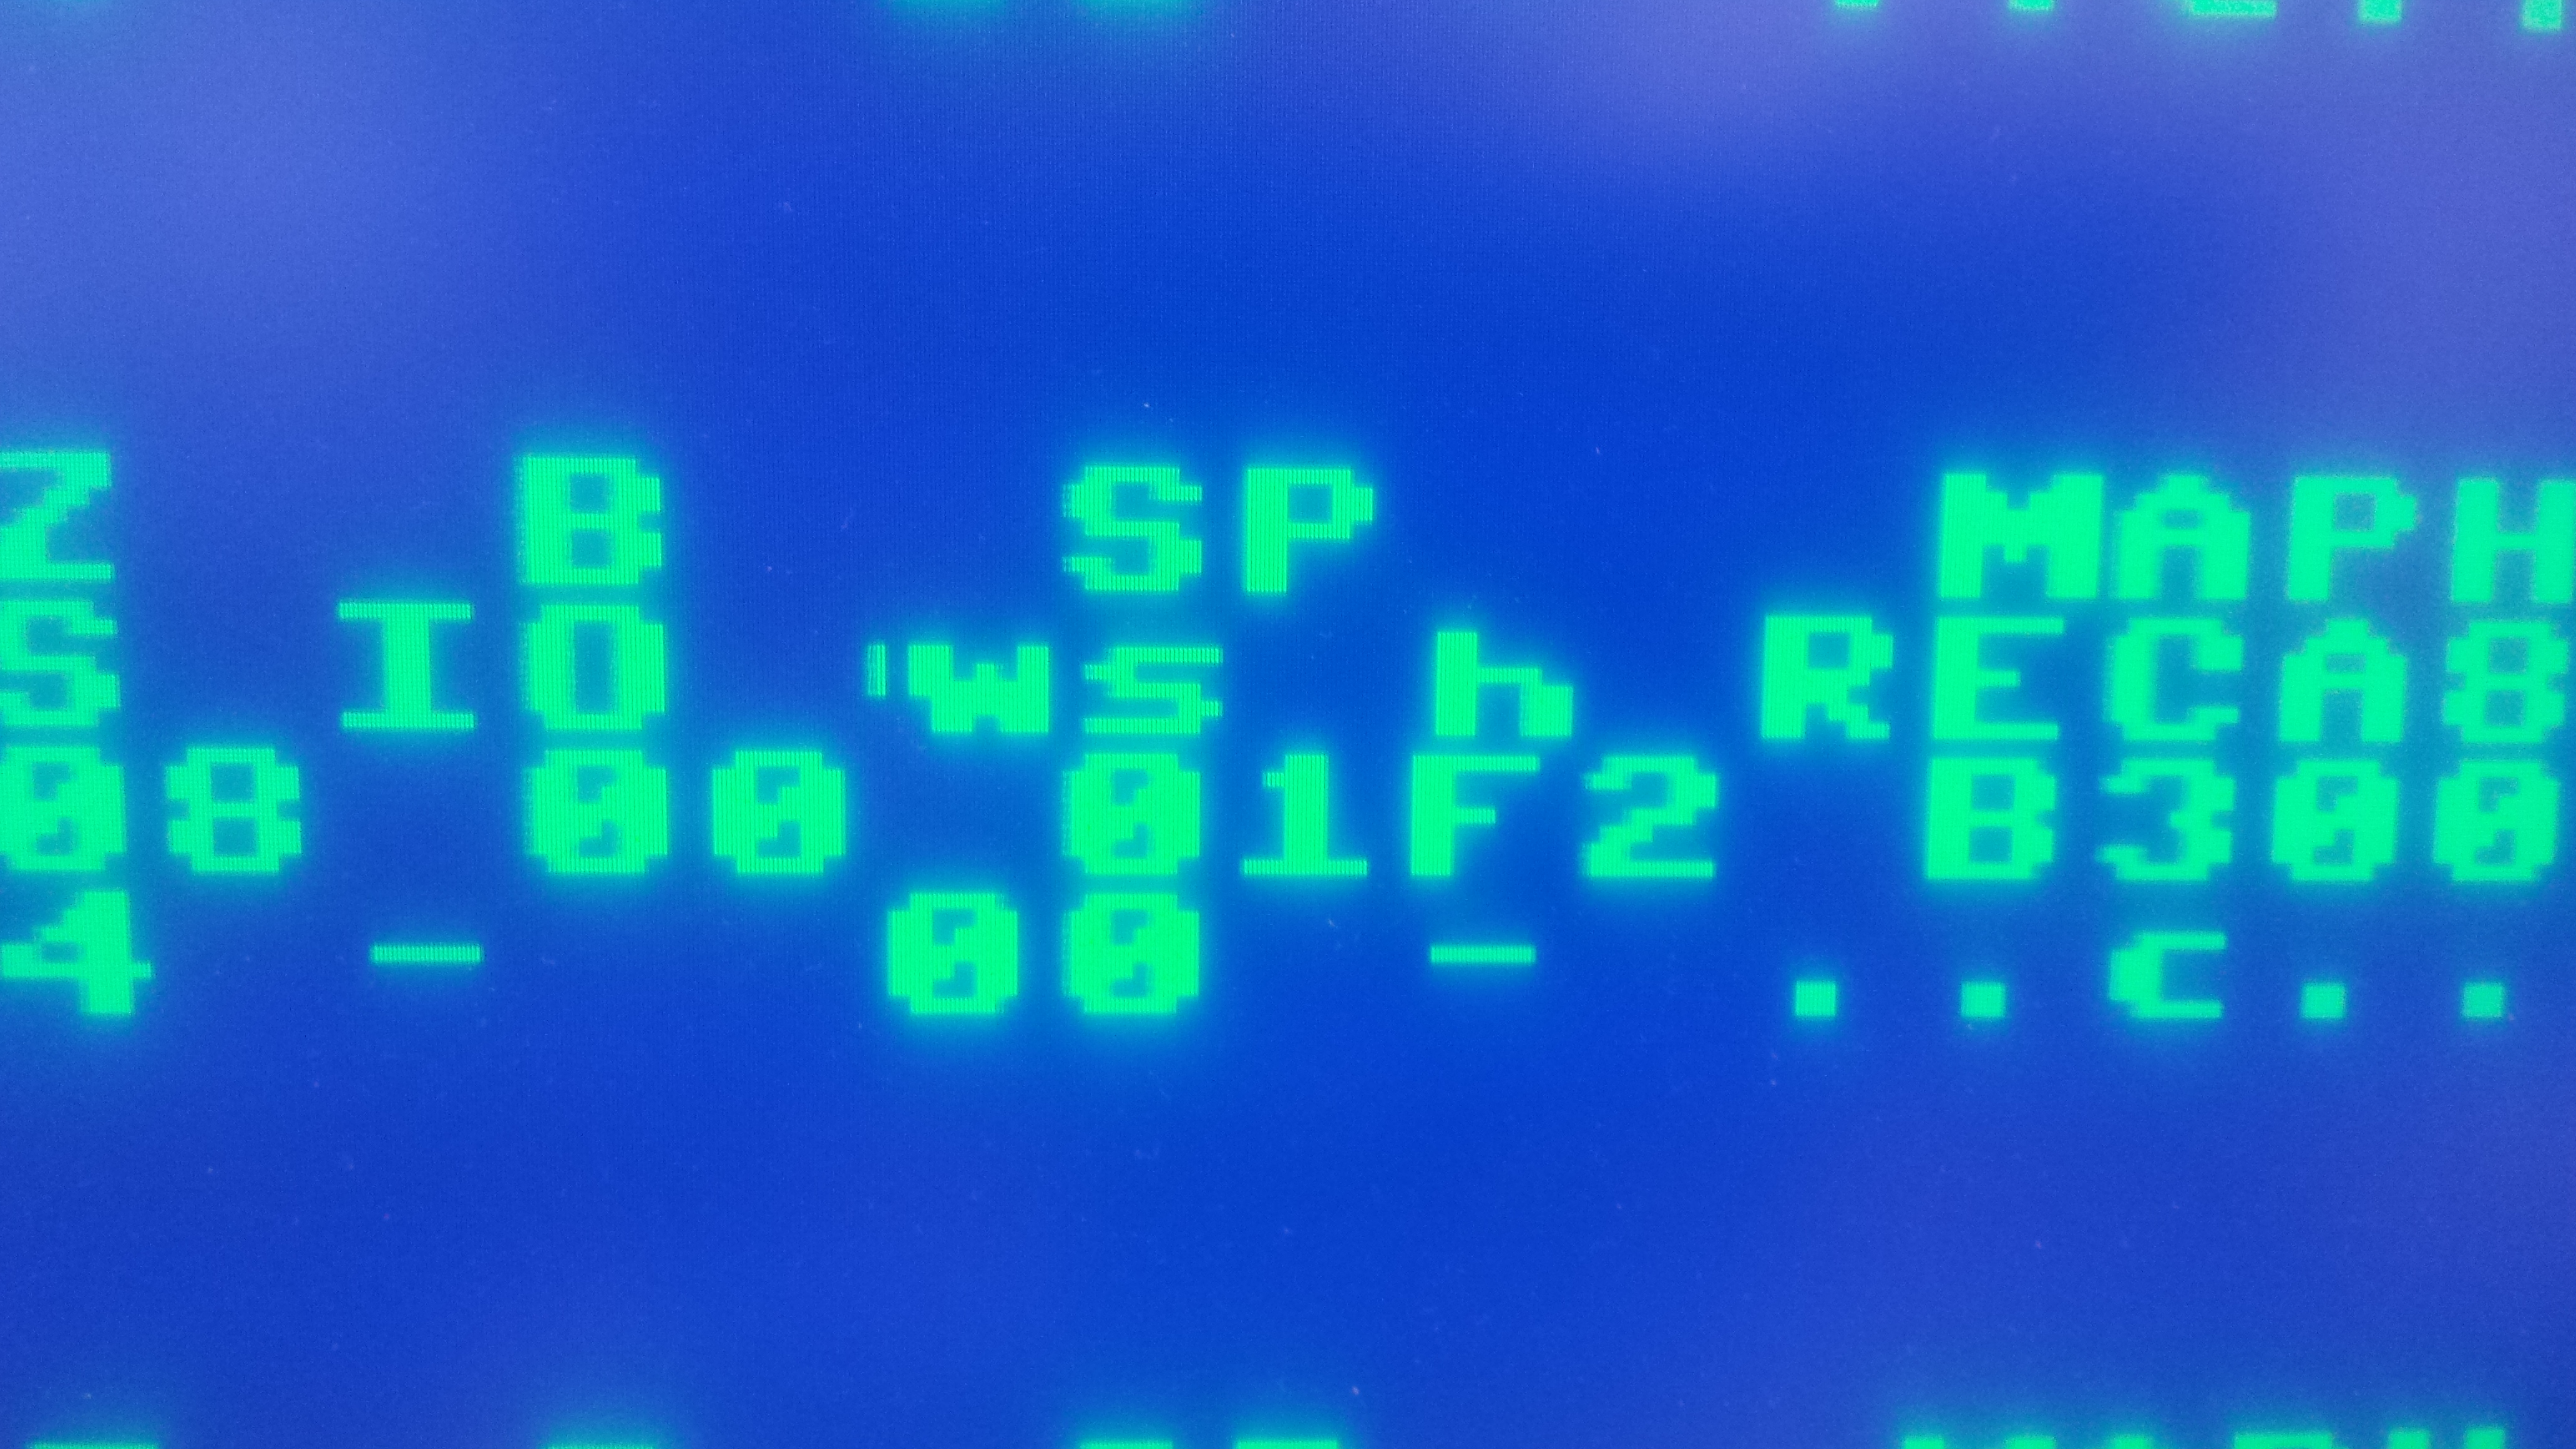
\includegraphics[width=\linewidth]{biterror}
  \caption{The matrix mode character shift.}
  \label{fig:biterror}
\end{figure}

\begin{figure}
  \centering
  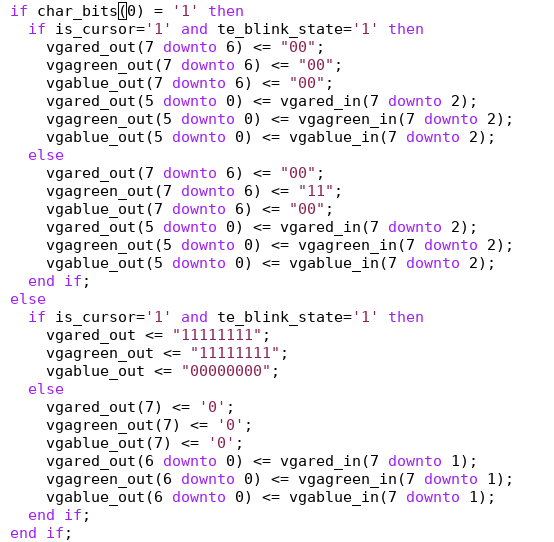
\includegraphics[width=\linewidth]{charbitstwo}
  \caption{The character bits to vga output code.}
  \label{fig:charbitstwo}
\end{figure}

\begin{figure}
  \centering
  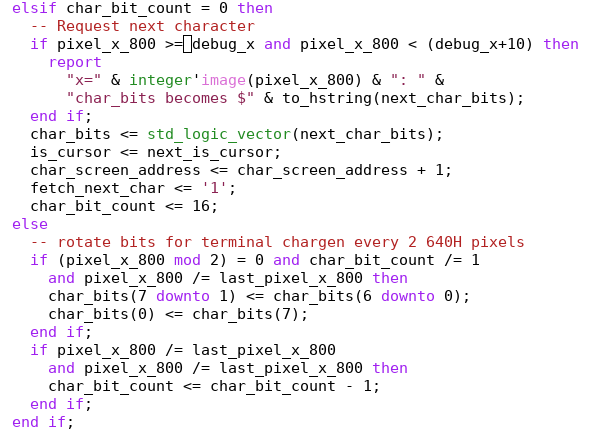
\includegraphics[width=\linewidth]{charbits}
  \caption{The character bit rotation code.}
  \label{fig:charbits}
\end{figure}

\begin{figure}
  \centering
  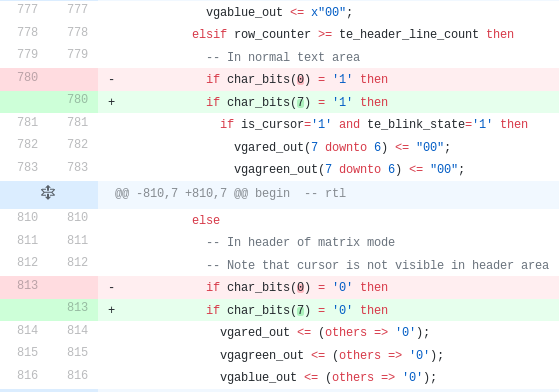
\includegraphics[width=\linewidth]{bitfix}
  \caption{The manual bit shift to counter the shifting error.}
  \label{fig:bitfix}
\end{figure}

%-----------------------------------
%	SUBSECTION 4
%-----------------------------------

\subsection{Letterbox Fixing}

\label{Ch5 Sec3 Sub4}

In collaboration with Dr. Gardner-Stephen, the junk characters seen at the bottom section of matrix mode, as seen if figure \ref{fig:letterbox}, were able to be restricted from the display. To perform this restriction of the output to the visible section of the screen, the row counter variable was used to determine if the current row was beyond the end of the matrix mode display. As seen in figure \ref{fig:letterboxfixtwo}, if the current row was beyond the end of the writeable matrix mode display, the vga input was darkened and passed out. This would hard code out any possibility of the matrix mode display being corrupted by junk characters being present in the terminal memory due to other faults.

\begin{figure}
  \centering
  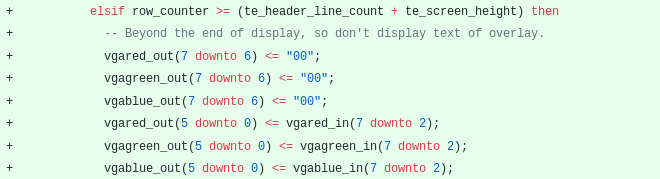
\includegraphics[width=\linewidth]{letterboxfixtwo}
  \caption{Correction to the rain compositor to stop the junk characters appearing in the lower section of the screen.}
  \label{fig:letterboxfixtwo}
\end{figure}

%-----------------------------------
%	SUBSECTION 5
%-----------------------------------

\subsection{Character Duplication}

\label{Ch5 Sec3 Sub5}

After letterbox implementation as described in section \ref{Ch5 Sec2}, a strange phenomenon occurred on the left side of the screen when in matrix mode. It appears that there is a region, about four character wide, that contains duplicates of characters from the next line. In addition to this duplicate, there appears to be smearing of the first two characters in this duplicate region. These observations can be seen in figure \ref{fig:matrixmodecharacterinputerror}. In addition to the issues with the left region, it is believed that these issues are causing the screen to become shifted to the right. As seen in figure \ref{fig:matrixmodecharacterinputerror}, the last four characters of the line are continuing past the right most visible point of the screen. 

\begin{figure}
  \centering
  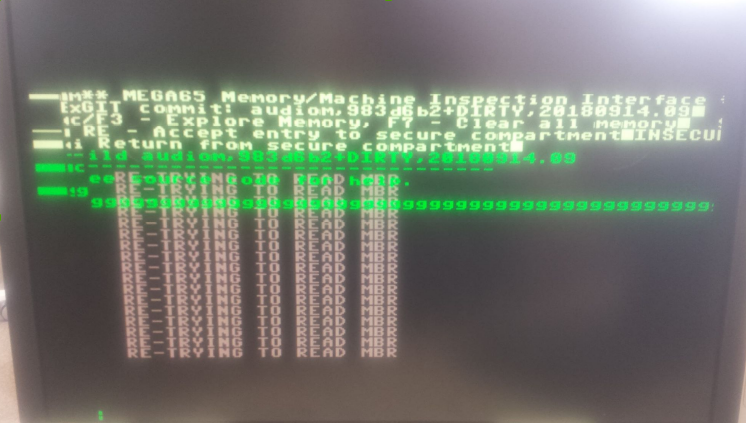
\includegraphics[width=\linewidth]{matrixmodecharacterinputerror}
  \caption{The matrix rain compositor smearing / duplication.}
  \label{fig:matrixmodecharacterinputerror}
\end{figure}
 
% Chapter Template

\chapter{Secure Compartmentalisation} % Main chapter title

\label{Chapter 6} % Change X to a consecutive number; for referencing this chapter elsewhere, use \ref{ChapterX}

This chapter goes over the frame work for how secure compartments will be implemented in the MEGA65. It will then discuss the problems encountered during the implementation of the secure compartments. Finally this chapter will talk about the possible issues with the secure compartments.

%----------------------------------------------------------------------------------------
%	SECTION 1
%----------------------------------------------------------------------------------------

\section{Theorised Operation}

\label{Ch6 Sec1}

Thanks to the work of Tim Kirby, a frame work was provided for the operation of the secure compartments of the phone, as seen in figure \ref{fig:timkirby}. From this diagram, the finite state machine seen in figure \ref{fig:securecompartmentsfsm} was created and the state transition actions were noted. As seen in both figures \ref{fig:timkirby} and \ref{fig:securecompartmentsfsm}, initially the user begins in the insecure user mode. This user mode is then halted via a hypervisor trap that causes the io registers and the RAM and ROM of the phone to be saved to the SD card. The non-transfer section of RAM and all of ROM are then erased. From one of the save-state slots on the SD card, the desired secure service is then loaded into ROM. As soon as this is finished matrix mode is triggered, the hypervisor is left and the CPU is halted. Matrix mode causes all external input into the phone, apart from the keyboard, to be cut off. At this point the user is able to inspect ROM and the transfer area of RAM. If the user is satisfied, by typing "ACCEPT" the secure service is then allowed to execute with the data provided in the transfer area of RAM. If the user is dissatisfied, by typing "REJECT" the secure service is erased from ROM, matrix mode is then left, the hypervisor is retriggered and the CPU is resumed. The hypervisor then uses the save-state created immediately prior to entering matrix mode to restore the io registers and load all the data that was saved back into RAM and ROM. If the secure container was accepted, any additional trap to the hypervisor will be seen as an exit request from the secure container. During an exit request, the user will once again be prompted to inspect the transfer area of RAM and then accept or reject the escaping of the of that data from the secure container. If satisfied, by typing "ACCEPT" the non-transfer section if RAM and all of ROM are once again erased. Then, identically to the user rejecting entry into the secure container, matrix mode is left, the hypervisor is retriggered and the CPU is resumed. The hypervisor then loads the save-state created immediately prior to entering matrix mode from the SD card, which is used to restore the io registers and reload data back into non-transfer RAM and ROM. If the user is dissatisfied with data escaping the secure container, by typing "REJECT" all of RAM and all of ROM are erased before the matrix mode exit. Then the save-state is loaded identically to the accepted exit case by the hypervisor and the resumed CPU. Finally, an exit status flag is raised depending on how the secure service transaction went.

\begin{figure}
  \centering
  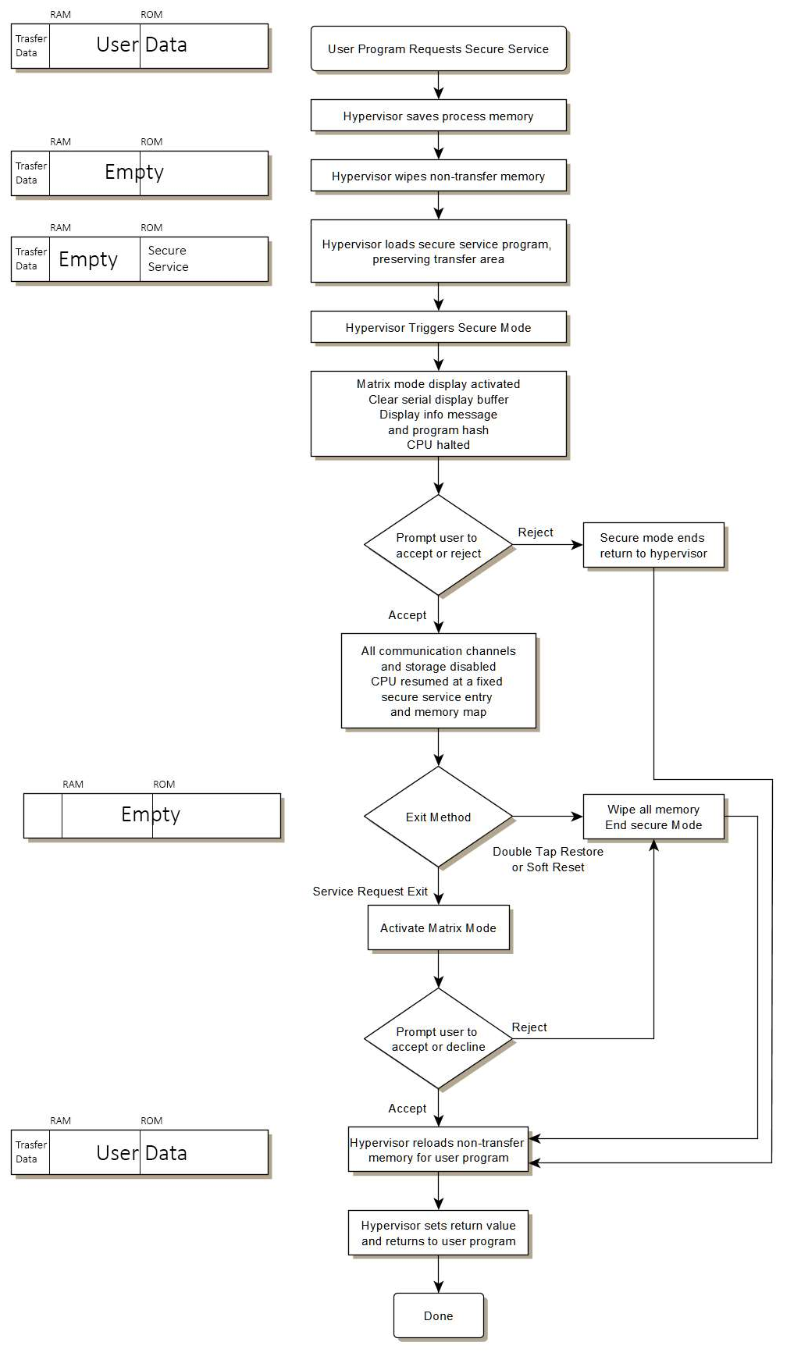
\includegraphics[width=\linewidth]{timkirby}
  \caption{The secure compartment frame work provided by Tim Kirby's thesis "Design and Development of a Secure Compartmentalised 8-bit Architecture".}
  \label{fig:timkirby}
\end{figure}

\begin{figure}
  \centering
  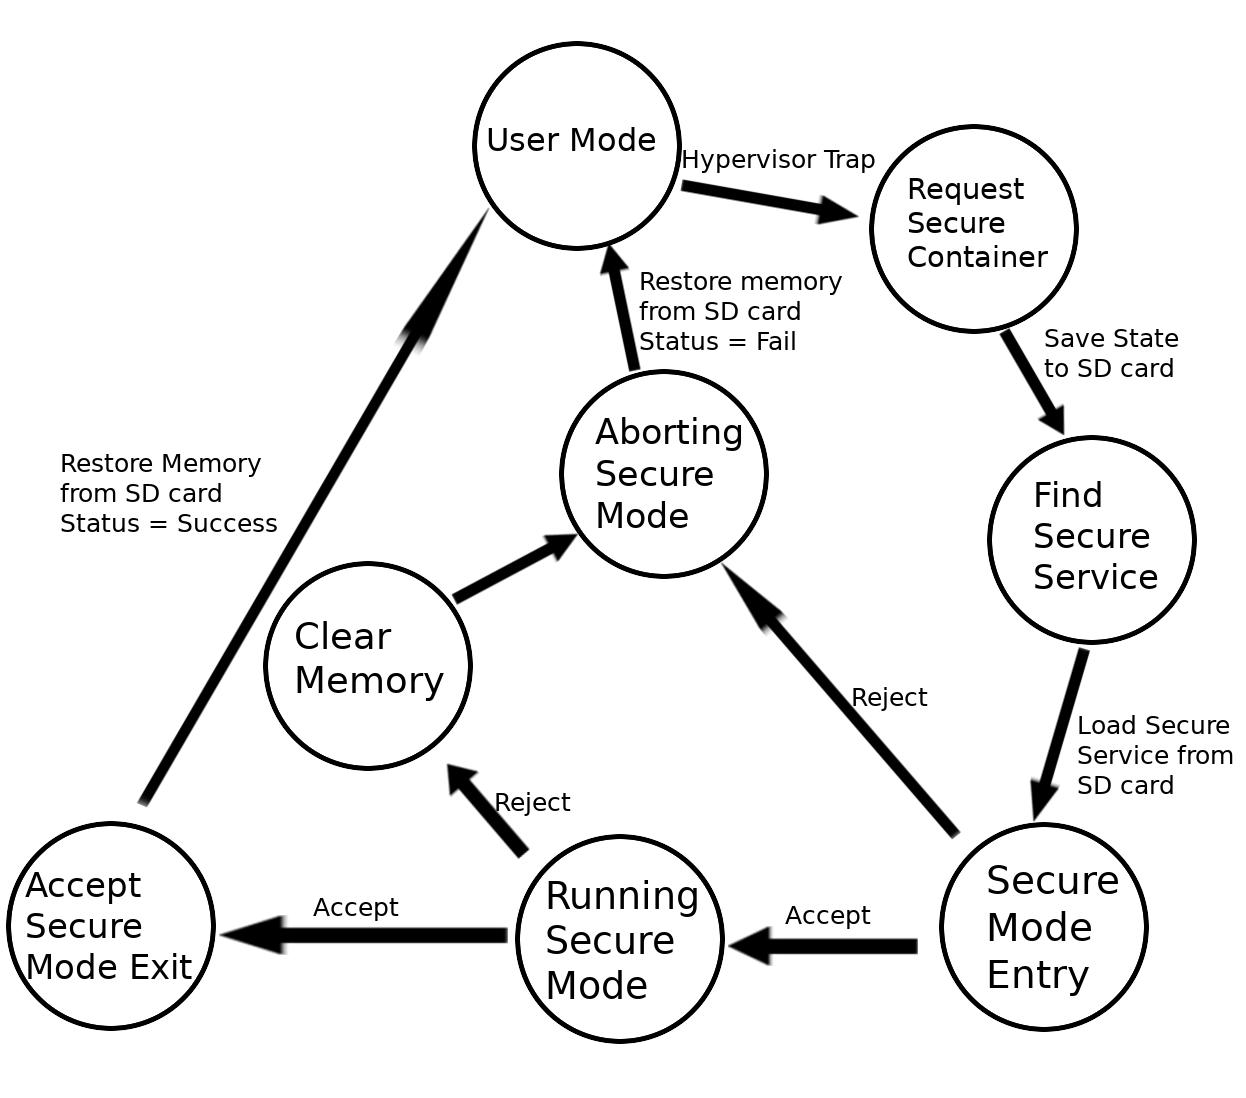
\includegraphics[width=\linewidth]{securecompartmentfsm}
  \caption{}
  \label{fig:securecompartmentsfsm}
\end{figure}

%----------------------------------------------------------------------------------------
%	SECTION 2
%----------------------------------------------------------------------------------------

\section{Initial Issues}

\label{Ch6 Sec2}

As the secure compartments were entirely separate from the matrix mode corrections and during the time a major update for another section of the phone was finished, a new branch of the project was created. Switching to this new branch resulted in overhead issues that needed to be solved in order for the project to proceed further.

%-----------------------------------
%	SUBSECTION 1
%-----------------------------------
\subsection{Repairing the Branch}

\label{Ch6 Sec2 Sub1}

As a new section of the project was being worked on the by other developers in isolation from the changes I had made, many of the fixes I had implemented had to be redone.\\
The timing fixes done to possibly correct the matrix mode issue were all removed, including the generation of the timing reports, these were reimplemented. The implementation was identical to that described in section \ref{Ch5 Sec1 Sub2} of chapter \ref{Chapter 5}.\\
All of the letterboxing changes were lost, so, as seen in section \ref{Ch5 Sec2} of chapter \ref{Chapter 5}, the erasing of the second character set was done one gains and the letterbox signal was one again used to limit the output of matrix mode.\\
The revolving line issue due to discrepancies in line length returned as was fixed as described in section \ref{Ch5 Sec3 Sub1} of chapter \ref{Chapter 5}.\\

In addition to the minor issues, matrix mode was not behaving as intended again. When attempting to enter or exit matrix mode with the tab + C= key combination, the key combination would be read and re-read rapidly and continuously. This made entering and exiting matrix mode unreliable as it was up to luck whether the key combination was scanned an odd or even amount of times to determine if the state was toggled. Tracing the matrix mode hypervisor trap from the CPU to the io mapper shows, as seen in figure \ref{fig:mmlatch}, there are latching and unlatching conditions for the matrix mode hypervisor trap. When monitoring the ascii\_key\_valid and ef\_latch signals via oscilloscope, the cause of the issue was clear. The ascii\_key\_valid signal was not a latching signal, and thus, it would only be high for a single clock cycle. As seen in the logic in figure \ref{fig:mmlatch}, this would cause the latch signal to pulse similarly, allowing the matrix mode hyper trap to be triggered every second clock cycle. A quick solution to this issue, as seen in figure \ref{fig:traptimeout} was written by Dr. Gardner-Stephen in the form of a timeout clock that blocks repeated instances of tab + C= from triggering the matrix mode hypervisor trap.

\begin{figure}
  \centering
  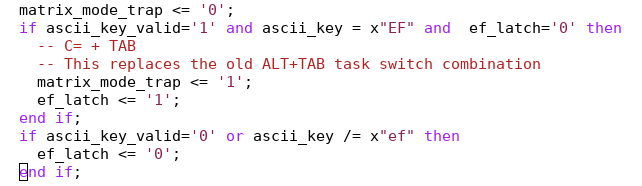
\includegraphics[width=\linewidth]{mmlatch}
  \caption{The matrix mode hypervisor trap latch.}
  \label{fig:mmlatch}
\end{figure}

\begin{figure}
  \centering
  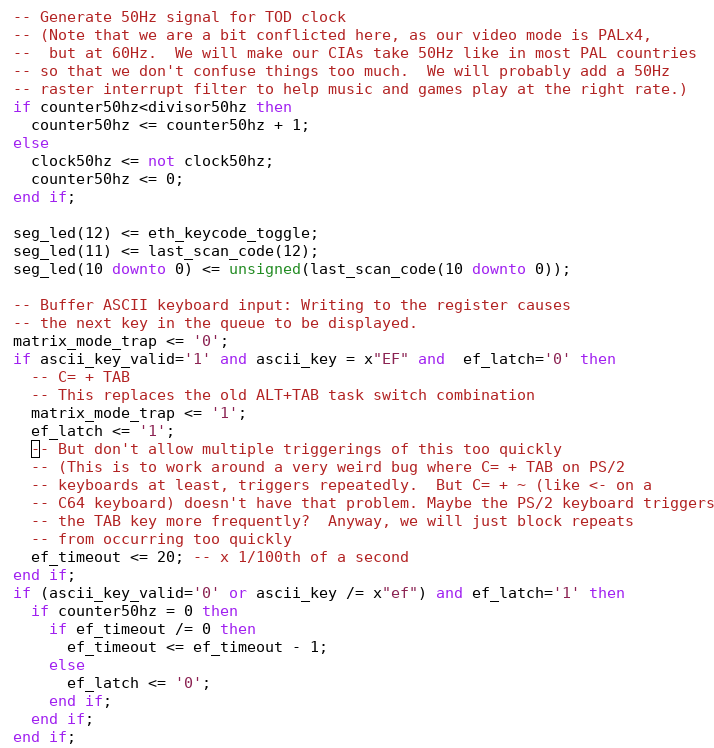
\includegraphics[width=\linewidth]{traptimeout}
  \caption{The matrix mode hypervisor trap latch with the new timeout period to prevent constant triggering.}
  \label{fig:traptimeout}
\end{figure}

%-----------------------------------
%	SUBSECTION 2
%-----------------------------------
\subsection{SD Card Restoration}

\label{Ch6 Sec2 Sub2}

One of the already implemented functions on the phone was the freeze function, this allowed the user to save state to a "Slot" located on the SD card. This freeze function would be the basis for the saving to and loading from the SD card when entering and exiting secure mode. The functionality for the standard capacity SD cards (SDSC) was entirely as expected, it was only the high capacity SD cards (SDHC) that were causing issues. When attempting to write to an SDHC card with the existing code, no visible errors occurred. It was only when attempting to read from this card that an issue occurred. When attempting to read after the first time the SD card would read no data, each read required a reset of the SD card between them in order for correct functionality. The extreme capacity SD card (SDXC) was not supported by the current hardware and indeed, was not recognised as an SD card at all when reading and writing was attempted. At the suggestion of Dr. Garner-Stephen, the issue with the SDHC cards was examined from the finite state machine located in the sdcard.vhdl file. As seen in figure \ref{fig:sdcardread} when reading or writing, the SD card is selected by making the cs\_bo bit low, and when it is not doing either of them, it is deselected by making cs\_bo high. Comparing this to the reset process seen in figures \ref{fig:resetsdcard}, \ref{fig:startsdcard} and \ref{fig:deselectsdcard}, it can be seen that there are several signals that are not being propagated when deselecting the SD card. At the suggestion of Dr. Gardner-Stephen, the simple solution of not deselecting the SD card was used. This solution, as seen in figure \ref{fig:sdcardfix}, does not provide hot swapping of the SD card, but has the functionality required for the secure mode implementation.

\begin{figure}
  \centering
  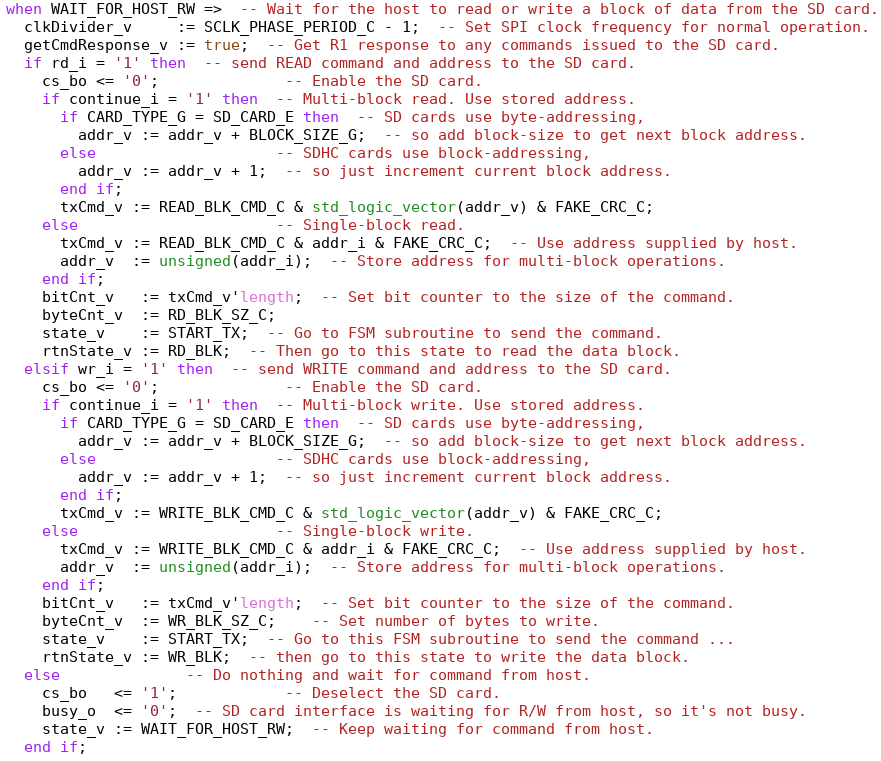
\includegraphics[width=\linewidth]{sdcardread}
  \caption{The SD card idle state code.}
  \label{fig:sdcardread}
\end{figure}

\begin{figure}
  \centering
  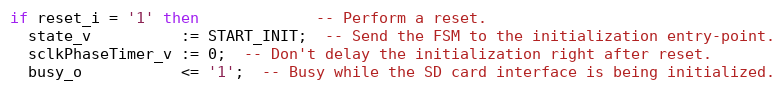
\includegraphics[width=\linewidth]{resetsdcard}
  \caption{The reset SD card code.}
  \label{fig:resetsdcard}
\end{figure}

\begin{figure}
  \centering
  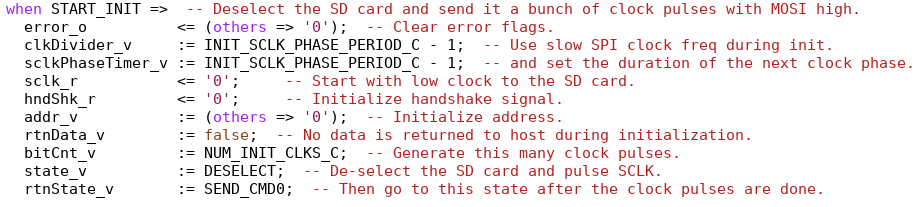
\includegraphics[width=\linewidth]{startsdcard}
  \caption{The SD card initial start up code.}
  \label{fig:startsdcard}
\end{figure}

\begin{figure}
  \centering
  \includegraphics[width=\linewidth]{deselectsdcard}
  \caption{The deselect SD card code.}
  \label{fig:deselectsdcard}
\end{figure}

\begin{figure}
  \centering
  \includegraphics[width=\linewidth]{sdcardfix}
  \caption{The fixed read, write and idle code for the SD card controller.}
  \label{fig:sdcardfix}
\end{figure}

%----------------------------------------------------------------------------------------
%	SECTION 3
%----------------------------------------------------------------------------------------

\section{Secure Compartment Implementation}

\label{Ch6 Sec3}

%-----------------------------------
%	SUBSECTION 1
%-----------------------------------

\subsection{Secure Mode Trap}

\label{Ch6 Sec3 Sub1}

As discussed in section \ref{Ch6 Sec1}, in order for the user to enter secure mode a hypervisor trap needs to be sent to the CPU. All hypervisor traps work in a single standard way, a set of conditions, usually a key combination, pulls the hypervisor trap signal low. This signal is then fed out of the triggering hardware where it is combined with the the other hypervisor traps to form a singular, active low, hypervisor trap. This hypervisor trap signal, seen in figure \ref{fig:hypervisortrap}, is then sent to the CPU, where it is used to determine the type of hypervisor trap occurring. As seen in figure \ref{fig:hypertrappending}, this trap input is then used to generate an edge signal which is further used to latch the hypervisor trap pending signal. This prevents the hypervisor trap from being lost if not active for long enough. This is then used in figure \ref{fig:enterhypervisor} to cause the next instruction of the CPU to enter the hypervisor mode. When entering the hypervisor the secure mode bit is checked to see if secure mode is already active, this is used for exiting secure mode and further discussed in section \ref{Ch6 Sec3 Sub4}. As seen in figure \ref{fig:hypertraptype}, when not in secure mode, the hypervisor\_trap\_port signal is used as a pointer to set the program counter to the desired hypervisor trap location in memory. These memory locations start at \$8000 and the secure mode trap is trap 11, which starts at memory location \$8044 and can be seen in figure \ref{fig:hypertrapsoftware}. This location in memory is where the next stage of the secure mode process, as described in section \ref{Ch6 Sec3 Sub2}, will take place.

\begin{figure}
  \centering
  \includegraphics[width=\linewidth]{hypervisortrap}
  \caption{The combining of the keyboard hypervisor trap and the monitor hypervisor trap.}
  \label{fig:hypervisortrap}
\end{figure}

\begin{figure}
  \centering
  \includegraphics[width=\linewidth]{hypertrappending}
  \caption{The hypervisor trap edge generation, pending trap generation and special trap input generation.}
  \label{fig:hypertrappending}
\end{figure}

\begin{figure}
  \centering
  \includegraphics[width=\linewidth]{enterhypervisor}
  \caption{The use of the hyper\_trap\_pending flag to enter the hypervisor mode.}
  \label{fig:enterhypervisor}
\end{figure}

\begin{figure}
  \centering
  \includegraphics[width=\linewidth]{hypertraptype}
  \caption{The statement that determines the type of hypervisor trap while entering hypervisor mode.}
  \label{fig:hypertraptype}
\end{figure}

\begin{figure}
  \centering
  \includegraphics[width=\linewidth]{hypertrapsoftware}
  \caption{The secure mode hypervisor trap service call.}
  \label{fig:hypertrapsoftware}
\end{figure}

%-----------------------------------
%	SUBSECTION 2
%-----------------------------------

\subsection{Save and Load State}

\label{Ch6 Sec3 Sub2}

Once trapped to the hypervisor, as described in section \ref{Ch6 Sec1} and seen in figure \ref{fig:timkirby}, the io registers, RAM and ROM all need to be saved to a save state slot. Upon entering the hypervisor, as seen in figure

\begin{figure}
  \centering
  \includegraphics[width=\linewidth]{hypertrapsoftwareone}
  \caption{}
  \label{fig:hypertrapsoftwareone}
\end{figure}

\begin{figure}
  \centering
  \includegraphics[width=\linewidth]{hypertrapsoftwaretwo}
  \caption{}
  \label{fig:hypertrapsoftwaretwo}
\end{figure}

%-----------------------------------
%	SUBSECTION 3
%-----------------------------------

\subsection{Secure Mode Entry}

\label{Ch6 Sec3 Sub3}

With the io registers, RAM and ROM all saved and the secure service loaded into RAM and ROM while preserving the transfer area, entry into secure mode can begin. This starts with the hypervisor toggling the secure mode and matrix mode bits of the protected hardware flags. As soon as there is a mismatch between the monitor secure mode flag and the CPU secure mode flag, as seen in figure \ref{fig:cpuhalt} the CPU is halted. This allows the secure mode signal to propagate out of the CPU to the monitor.\\

The monitor, as opposed to the Intel Management Engine (IME) service CPU, is a servant CPU. The key difference between the two being that where the IME is able to autonomously perform commands, whereas the monitor CPU requires the user to issue commands. The monitor CPU was introduced due to hardware limitations of the FPGA. Previously the monitor was entirely hardware with no CPU at all, this took up lots of space on the FPGA and would prevent the rest of the phone from being able to fit. By converting the monitor into a servant CPU the large amount of specialised hardware was able to be condensed into a multipurpose unit.\\

As seen in figure \ref{fig:monitorprotectedhardware}, when the secure mode flag reaches the monitor CPU, it is eventually scanned and used to branch and enter the secure mode routine. In this routine, as seen in figure \ref{fig:maybeentersecuremode}, currently only the local secure mode variable is set high and the routine returns to figure \ref{fig:monitorprotectedhardware}. In the future iterations, an indicator as to how much memory the transfer area occupies will need to be implemented.\\

In parallel to the monitor functions, the protected hardware signal is fed into the matrix mode compositor. This displays the secure mode screen entirely independently from the secure mode verification and locks down the inputs and outputs from the MEGA65. Once the monitor CPU verification has completed, as seen in figure \ref{fig:monitoracceptreject} the user is required to enter "ACCEPT" or "REJECT" to approve or disapprove entry into the secure container. In the "ACCEPT" case, this will parse the local secure mode variable out and to the CPU. In the "REJECT" case, the io registers, RAM and ROM are be restored from the save state created in section \ref{Ch6 Sec3 Sub3} and then the local variable for secure mode will be parsed to the CPU. The "ACCEPT" case can be seen in figure \ref{fig:monitoraccept} and the "REJECT" case can be seen in figure \ref{fig:monitorreject}.\\

While the "ACCEPT" case has been fully implemented, the "REJECT" case has not been implemented at all. Figure \ref{fig:monitorreject} shows that in the "REJECT" case, all that is occuring is the memory is being erased before the local secure mode value is sent out of the monitor.\\ %% XXX -- ASK PAUL ABOUT THE SECURE MODE REJECT ROUTINE ONCE THE MONITOR HAS RECIEVED THE REJECT COMMAND %%

Once the input has been read and either the "ACCEPT" case or the "REJECT" case has been recognised and acted upon, the monitor will then leave the matrix mode screen, as seen in figure \ref{fig:monitoraccept}. In addition to leaving the matrix mode screen, the CPU is unhalted, this allows the secure service or loaded save state to function.

\begin{figure}
  \centering
  \includegraphics[width=\linewidth]{monitorprotectedhardware}
  \caption{The routine that checks the protected hardware to determine if the phone should be in secure mode}
  \label{fig:monitorprotectedhardware}
\end{figure}

\begin{figure}
  \centering
  \includegraphics[width=\linewidth]{maybeentersecuremode}
  \caption{The routine that sets the secure mode flag to non-zero value.}
  \label{fig:maybeentersecuremode}
\end{figure}

\begin{figure}
  \centering
  \includegraphics[width=\linewidth]{cpuhalt}
  \caption{The CPU halting code that halts when the CPU and monitor disagree on if the phone is in secure mode.}
  \label{fig:cpuhalt}
\end{figure}

\begin{figure}
  \centering
  \includegraphics[width=\linewidth]{monitoracceptreject}
  \caption{The monitor CPU code that compares the input string against a string containing "ACCEPT" and one containing "REJECT".}
  \label{fig:monitoracceptreject}
\end{figure}

\begin{figure}
  \centering
  \includegraphics[width=\linewidth]{monitoraccept}
  \caption{The monitor CPU "ACCEPT" case.}
  \label{fig:monitoraccept}
\end{figure}

\begin{figure}
  \centering
  \includegraphics[width=\linewidth]{monitorreject}
  \caption{The monitor CPU "REJECT" case.}
  \label{fig:monitorreject}
\end{figure}

%-----------------------------------
%	SUBSECTION 4
%-----------------------------------

\subsection{Secure Mode Exit}

\label{Ch6 Sec3 Sub4}

While in secure mode, any hypervisor trap will be seen as a request for exit from secure mode. This, as seen in figure \ref{fig:securemodeexit}, overwrites the hypervisor trap determination seen in figure \ref{fig:enterhypervisor} with the exact location of the exit secure mode trap and sets the matrix mode flag high and secure mode flag low. Once again the CPU is halted due to the mismatch seen in figure \ref{fig:cpuhalt} between the monitor secure mode state and the CPU secure mode state.\\

The code seen in figure \ref{fig:monitorprotectedhardware} is once again run, but this time branches to figure \ref{fig:monitorleavesecuremode}. As in section \ref{Ch6 Sec3 Sub3}, while the monitor CPU is performing the verification check, the matrix mode compositor is displaying the secure mode exit screen and prompting the user to enter "ACCEPT" or "REJECT". As seen in figures \ref{fig:monitoracceptreject} and \ref{fig:monitoraccept}, in the "ACCEPT" case the CPU is allowed to run by setting the monitor secure mode state to be identical to the CPU. In the "REJECT" case, demonstraited by figure \ref{fig:monitorreject},  all the top megabyte of address space is erased and io address registers are also erased.\\

The "REJECT" case, as seen in figure \ref{fig:monitorerase}, has not entirely been implemented, in the future it needs to overwrite the RAM, ROM and io registers in addition to what it is already erasing. Once all the erasing has been done, the local secure mode flag needs to then be altered to allow the CPU to run again.\\

Like the "REJECT" case, the "ACCEPT" case needs to be fully implemented. Currently, accepting a leave request from secure mode allows all memory to escape the secure container. In future development, the io registers, ROM and non-transfer area RAM need to be erased.

\begin{figure}
  \centering
  \includegraphics[width=\linewidth]{securemodeexit}
  \caption{The CPU hypervisor trap determination code.}
  \label{fig:securemodeexit}
\end{figure}

\begin{figure}
  \centering
  \includegraphics[width=\linewidth]{monitorleavesecuremode}
  \caption{The monitor CPU leave secure mode routine.}
  \label{fig:monitorleavesecuremode}
\end{figure}

\begin{figure}
  \centering
  \includegraphics[width=\linewidth]{monitorerase}
  \caption{The monitor CPU erase routine.}
  \label{fig:monitorerase}
\end{figure}

%-----------------------------------
%	SUBSECTION 5
%-----------------------------------

\subsection{Restore User Mode}

\label{Ch6 Sec3 Sub5}

Once either "ACCEPT" or "REJECT" has occured and the CPU is running again, the hypervisor will then 


%% Put this in section 2

%\subsection{Secure Compartment Issue}

%\label{Ch6 Sec1 Sub1}

%During the development of the secure compartments, an issue with the design was made apparent. As explained in the previous section, when entering or exiting secure mode the hypervisor is in complete control of the phone's operation. This poses a problem if it were to experiance any subversion. Between the loading of the secure service and the entering of secure mode and halting of the CPU, there is opportunity for the 

% Chapter Template

\chapter{Results and Discussion} % Main chapter title

\label{Chapter 7} % Change X to a consecutive number; for referencing this chapter elsewhere, use \ref{ChapterX}

%----------------------------------------------------------------------------------------
%	SECTION 1
%----------------------------------------------------------------------------------------

\section{Main Section 1}

%% Look back at what was achieved and comment on the research questions. How they were answered, fully yes fully no, partially?

%-----------------------------------
%	SUBSECTION 1
%-----------------------------------
\subsection{Subsection 1}

Nunc posuere quam at lectus tristique eu ultrices augue venenatis. Vestibulum ante ipsum primis in faucibus orci luctus et ultrices posuere cubilia Curae; Aliquam erat volutpat. Vivamus sodales tortor eget quam adipiscing in vulputate ante ullamcorper. Sed eros ante, lacinia et sollicitudin et, aliquam sit amet augue. In hac habitasse platea dictumst.

%-----------------------------------
%	SUBSECTION 2
%-----------------------------------

\subsection{Subsection 2}
Morbi rutrum odio eget arcu adipiscing sodales. Aenean et purus a est pulvinar pellentesque. Cras in elit neque, quis varius elit. Phasellus fringilla, nibh eu tempus venenatis, dolor elit posuere quam, quis adipiscing urna leo nec orci. Sed nec nulla auctor odio aliquet consequat. Ut nec nulla in ante ullamcorper aliquam at sed dolor. Phasellus fermentum magna in augue gravida cursus. Cras sed pretium lorem. Pellentesque eget ornare odio. Proin accumsan, massa viverra cursus pharetra, ipsum nisi lobortis velit, a malesuada dolor lorem eu neque.

%----------------------------------------------------------------------------------------
%	SECTION 2
%----------------------------------------------------------------------------------------

\section{Main Section 2}

Sed ullamcorper quam eu nisl interdum at interdum enim egestas. Aliquam placerat justo sed lectus lobortis ut porta nisl porttitor. Vestibulum mi dolor, lacinia molestie gravida at, tempus vitae ligula. Donec eget quam sapien, in viverra eros. Donec pellentesque justo a massa fringilla non vestibulum metus vestibulum. Vestibulum in orci quis felis tempor lacinia. Vivamus ornare ultrices facilisis. Ut hendrerit volutpat vulputate. Morbi condimentum venenatis augue, id porta ipsum vulputate in. Curabitur luctus tempus justo. Vestibulum risus lectus, adipiscing nec condimentum quis, condimentum nec nisl. Aliquam dictum sagittis velit sed iaculis. Morbi tristique augue sit amet nulla pulvinar id facilisis ligula mollis. Nam elit libero, tincidunt ut aliquam at, molestie in quam. Aenean rhoncus vehicula hendrerit.

% Chapter Template

\chapter{Conclusion} % Main chapter title

\label{Chapter 8} % Change X to a consecutive number; for referencing this chapter elsewhere, use \ref{ChapterX}

%----------------------------------------------------------------------------------------
%	SECTION 1
%----------------------------------------------------------------------------------------

\section{Main Section 1}

Lorem ipsum dolor sit amet, consectetur adipiscing elit. Aliquam ultricies lacinia euismod. Nam tempus risus in dolor rhoncus in interdum enim tincidunt. Donec vel nunc neque. In condimentum ullamcorper quam non consequat. Fusce sagittis tempor feugiat. Fusce magna erat, molestie eu convallis ut, tempus sed arcu. Quisque molestie, ante a tincidunt ullamcorper, sapien enim dignissim lacus, in semper nibh erat lobortis purus. Integer dapibus ligula ac risus convallis pellentesque.

%-----------------------------------
%	SUBSECTION 1
%-----------------------------------
\subsection{Subsection 1}

Nunc posuere quam at lectus tristique eu ultrices augue venenatis. Vestibulum ante ipsum primis in faucibus orci luctus et ultrices posuere cubilia Curae; Aliquam erat volutpat. Vivamus sodales tortor eget quam adipiscing in vulputate ante ullamcorper. Sed eros ante, lacinia et sollicitudin et, aliquam sit amet augue. In hac habitasse platea dictumst.

%-----------------------------------
%	SUBSECTION 2
%-----------------------------------

\subsection{Subsection 2}
Morbi rutrum odio eget arcu adipiscing sodales. Aenean et purus a est pulvinar pellentesque. Cras in elit neque, quis varius elit. Phasellus fringilla, nibh eu tempus venenatis, dolor elit posuere quam, quis adipiscing urna leo nec orci. Sed nec nulla auctor odio aliquet consequat. Ut nec nulla in ante ullamcorper aliquam at sed dolor. Phasellus fermentum magna in augue gravida cursus. Cras sed pretium lorem. Pellentesque eget ornare odio. Proin accumsan, massa viverra cursus pharetra, ipsum nisi lobortis velit, a malesuada dolor lorem eu neque.

%----------------------------------------------------------------------------------------
%	SECTION 2
%----------------------------------------------------------------------------------------

\section{Main Section 2}

Sed ullamcorper quam eu nisl interdum at interdum enim egestas. Aliquam placerat justo sed lectus lobortis ut porta nisl porttitor. Vestibulum mi dolor, lacinia molestie gravida at, tempus vitae ligula. Donec eget quam sapien, in viverra eros. Donec pellentesque justo a massa fringilla non vestibulum metus vestibulum. Vestibulum in orci quis felis tempor lacinia. Vivamus ornare ultrices facilisis. Ut hendrerit volutpat vulputate. Morbi condimentum venenatis augue, id porta ipsum vulputate in. Curabitur luctus tempus justo. Vestibulum risus lectus, adipiscing nec condimentum quis, condimentum nec nisl. Aliquam dictum sagittis velit sed iaculis. Morbi tristique augue sit amet nulla pulvinar id facilisis ligula mollis. Nam elit libero, tincidunt ut aliquam at, molestie in quam. Aenean rhoncus vehicula hendrerit.

% Chapter Template

\chapter{Conclusion} % Main chapter title

\label{Chapter 9} % Change X to a consecutive number; for referencing this chapter elsewhere, use \ref{ChapterX}

%----------------------------------------------------------------------------------------
%	SECTION 1
%----------------------------------------------------------------------------------------

\section{Main Section 1}

Lorem ipsum dolor sit amet, consectetur adipiscing elit. Aliquam ultricies lacinia euismod. Nam tempus risus in dolor rhoncus in interdum enim tincidunt. Donec vel nunc neque. In condimentum ullamcorper quam non consequat. Fusce sagittis tempor feugiat. Fusce magna erat, molestie eu convallis ut, tempus sed arcu. Quisque molestie, ante a tincidunt ullamcorper, sapien enim dignissim lacus, in semper nibh erat lobortis purus. Integer dapibus ligula ac risus convallis pellentesque.

%-----------------------------------
%	SUBSECTION 1
%-----------------------------------
\subsection{Subsection 1}

Nunc posuere quam at lectus tristique eu ultrices augue venenatis. Vestibulum ante ipsum primis in faucibus orci luctus et ultrices posuere cubilia Curae; Aliquam erat volutpat. Vivamus sodales tortor eget quam adipiscing in vulputate ante ullamcorper. Sed eros ante, lacinia et sollicitudin et, aliquam sit amet augue. In hac habitasse platea dictumst.

%-----------------------------------
%	SUBSECTION 2
%-----------------------------------

\subsection{Subsection 2}
Morbi rutrum odio eget arcu adipiscing sodales. Aenean et purus a est pulvinar pellentesque. Cras in elit neque, quis varius elit. Phasellus fringilla, nibh eu tempus venenatis, dolor elit posuere quam, quis adipiscing urna leo nec orci. Sed nec nulla auctor odio aliquet consequat. Ut nec nulla in ante ullamcorper aliquam at sed dolor. Phasellus fermentum magna in augue gravida cursus. Cras sed pretium lorem. Pellentesque eget ornare odio. Proin accumsan, massa viverra cursus pharetra, ipsum nisi lobortis velit, a malesuada dolor lorem eu neque.

%----------------------------------------------------------------------------------------
%	SECTION 2
%----------------------------------------------------------------------------------------

\section{Main Section 2}

Sed ullamcorper quam eu nisl interdum at interdum enim egestas. Aliquam placerat justo sed lectus lobortis ut porta nisl porttitor. Vestibulum mi dolor, lacinia molestie gravida at, tempus vitae ligula. Donec eget quam sapien, in viverra eros. Donec pellentesque justo a massa fringilla non vestibulum metus vestibulum. Vestibulum in orci quis felis tempor lacinia. Vivamus ornare ultrices facilisis. Ut hendrerit volutpat vulputate. Morbi condimentum venenatis augue, id porta ipsum vulputate in. Curabitur luctus tempus justo. Vestibulum risus lectus, adipiscing nec condimentum quis, condimentum nec nisl. Aliquam dictum sagittis velit sed iaculis. Morbi tristique augue sit amet nulla pulvinar id facilisis ligula mollis. Nam elit libero, tincidunt ut aliquam at, molestie in quam. Aenean rhoncus vehicula hendrerit.


%----------------------------------------------------------------------------------------
%	THESIS CONTENT - APPENDICES
%----------------------------------------------------------------------------------------

\appendix % Cue to tell LaTeX that the following "chapters" are Appendices

% Include the appendices of the thesis as separate files from the Appendices folder
% Uncomment the lines as you write the Appendices

%% Appendix A

\chapter{Frequently Asked Questions} % Main appendix title

\label{AppendixA} % For referencing this appendix elsewhere, use \ref{AppendixA}

\section{How do I change the colors of links?}

The color of links can be changed to your liking using:

{\small\verb!\hypersetup{urlcolor=red}!}, or

{\small\verb!\hypersetup{citecolor=green}!}, or

{\small\verb!\hypersetup{allcolor=blue}!}.

\noindent If you want to completely hide the links, you can use:

{\small\verb!\hypersetup{allcolors=.}!}, or even better: 

{\small\verb!\hypersetup{hidelinks}!}.

\noindent If you want to have obvious links in the PDF but not the printed text, use:

{\small\verb!\hypersetup{colorlinks=false}!}.

%\include{Appendices/AppendixB}
%\include{Appendices/AppendixC}

%----------------------------------------------------------------------------------------
%	BIBLIOGRAPHY
%----------------------------------------------------------------------------------------

\printbibliography[heading=bibintoc]

%----------------------------------------------------------------------------------------

\end{document}  
